%% CoopGCN --- Array (Elsevier) submission
%% Template: elsarticle.cls (Elsevier), single-column preprint, numbered references
%% Compile:  pdflatex coopgcn_array -> bibtex coopgcn_array -> pdflatex x2
\documentclass[preprint,12pt,authoryear]{elsarticle}

\usepackage{amsmath,amssymb,amsthm}
\usepackage{graphicx}
\usepackage{booktabs}
\usepackage{multirow}
\usepackage{url}
\usepackage[hidelinks]{hyperref}
\usepackage{xcolor}
\usepackage{algorithm}
\usepackage{algpseudocode}

\newtheorem{proposition}{Proposition}
\newtheorem{definition}{Definition}
\newtheorem{axiom}{Axiom}

\journal{Array}

\begin{document}

\begin{frontmatter}

\title{CoopGCN: Axiomatic Credit Assignment in Graph Convolutional
Networks via Tri-Level Cooperative Game Theory for Robust,
Preference-Aware Recommendation}

\author[inst1]{Mouad Louhichi\corref{cor1}}
\ead{mouad_louhichi@um5.ac.ma}
\author[inst1]{Redwane Nesmaoui}
\author[inst1]{Mohamed Lazaar}

\cortext[cor1]{Corresponding author.}

\affiliation[inst1]{organization={National Higher School of Computer Science and
Systems Analysis (ENSIAS), Mohammed V University in Rabat},
            city={Rabat},
            country={Morocco}}

\begin{abstract}
Linearised graph convolutional networks (GCNs) such as LightGCN have become the
default backbone for collaborative filtering by discarding feature
transformations and nonlinear activations. This simplification, however,
removes every mechanism for \emph{differential credit assignment}: each
neighbour contributes through a fixed topological coefficient
$1/\sqrt{d_u d_i}$, so a decade-old incidental rating and a recent niche
purchase propagate with identical relative importance. The consequences are
well documented---popularity-bias amplification, near-zero long-tail exposure,
and brittleness under noisy or adversarial edges. We argue that neighbourhood
aggregation in collaborative filtering is fundamentally a \emph{cooperative
credit-assignment game}, and we introduce \textbf{CoopGCN}, a recommender
framework that instantiates this view at three structural levels: an
edge-level game ($\mathbf{G_1}$) that modulates pairwise message weights by
Monte-Carlo Shapley values; a hyperedge-level game ($\mathbf{G_2}$) that
weights beyond-pairwise group coalitions; and a data-level game
($\mathbf{G_3}$) that applies truncated Monte-Carlo Shapley valuation to
reweight and prune training interactions. Because the Shapley value is the
unique allocation satisfying efficiency, symmetry, dummy-player and additivity,
credit assignment in CoopGCN is axiomatic rather than heuristic; in particular
the dummy-player axiom drives the weight of an uninformative edge to zero,
which we formalise as a bounded-perturbation guarantee. A Shapley consistency
loss $\mathcal{L}_{\mathrm{game}}$ distils exponential-moving-average Shapley
credits into learnable attention, so all game-theoretic computation is confined
to training and inference cost is unchanged. On ML-1M, Yelp2018 and
Amazon-Book under a full-catalogue ranking protocol at cut-off 20, CoopGCN
attains NDCG@20 of 0.2960, 0.0680 and 0.0480, improving on the strongest
baseline per dataset by 6.7\%, 13.1\% and 12.1\%, while raising catalogue
coverage by $4.2\times$, $16.6\times$ and $56.7\times$ over LightGCN and
reducing the Gini index on all three. Under 20\% adversarial edge injection
CoopGCN loses 5.4\% NDCG@20 on ML-1M against 25.0--29.0\% for all baselines.
A component ablation confirms that each of $\mathbf{G_1}$, $\mathbf{G_2}$,
$\mathbf{G_3}$ and the contrastive channel contributes positively, with
$\mathbf{G_1}$ the single largest contributor to tail recall.
\end{abstract}

\begin{keyword}
Recommender systems \sep Graph convolutional networks \sep Cooperative game
theory \sep Shapley value \sep Popularity bias \sep Long-tail recommendation
\sep Adversarial robustness
\end{keyword}

\end{frontmatter}

%==========================================================================
\section{Introduction}
\label{sec:intro}

Graph convolutional networks reshaped collaborative filtering (CF) by treating
the user--item interaction history as a bipartite graph over which preference
signal propagates. NGCF \citep{wang2019ngcf} established that high-order
connectivity carries exploitable information, and LightGCN
\citep{he2020lightgcn} subsequently demonstrated that the nonlinear activations
and feature-transformation matrices inherited from generic GCNs are not merely
unnecessary for pure CF but actively harmful, inducing oversmoothing and
training instability. Removing them yields the now-canonical propagation rule
\begin{equation}
\mathbf{E}^{(k+1)} = \left( \mathbf{D}^{-\frac{1}{2}} \mathbf{A}
\mathbf{D}^{-\frac{1}{2}} \right) \mathbf{E}^{(k)} ,
\label{eq:lightgcn}
\end{equation}
which remains a strong and remarkably durable empirical baseline.

The simplification came at an under-acknowledged architectural cost. In
Eq.~\eqref{eq:lightgcn} the influence of neighbour $i$ on user $u$ is fixed at
$w_{ui} = 1/\sqrt{d_u d_i}$, a quantity determined entirely by graph topology.
No component of the model can express that one interaction was informative and
another was noise. We identify four structural failure modes that follow
directly from this absence of credit assignment.

\begin{enumerate}
\item \textbf{Uniform neighbour weighting.} Every edge incident on a node is
trusted equally. A user's single accidental click on a blockbuster is weighted
by the same rule as a deliberate engagement with a niche title, and because the
coefficient is degree-normalised, high-degree items systematically dominate the
aggregate.

\item \textbf{No credit attribution.} The model cannot answer which historical
interactions produced a given recommendation. This is a limitation for
explainability, but it is equally a limitation for \emph{learning}: without a
notion of edge value there is no principled signal for denoising.

\item \textbf{Pairwise-only topology.} Bipartite edges encode $(u,i)$ relations
and cannot represent group structures---baskets, sessions, genre or category
bundles---that are natural units of preference. Hypergraph recommenders
\citep{xia2022hccf,chen2024hpcf} address this, but weight hyperedges by
heuristics or learned attention.

\item \textbf{Popularity-bias amplification.} Repeated convolution is dominated
by the leading eigenvectors of $\mathbf{A}$, contracting embeddings toward
high-degree items. Combined with BPR-style objectives under uniform negative
sampling, tail exposure collapses: in our evaluation, LightGCN, SGL, SimGCL,
HCCF and DyHuCoG all record TR@20 $= 0.0000$ on ML-1M while covering under
11\% of the catalogue.
\end{enumerate}

\subsection{Message passing as a cooperative game}

Our starting observation is that predicting a preference score
$s_{ui} = \bar{\mathbf{e}}_u^{\top} \bar{\mathbf{e}}_i$ is a \emph{team
production} problem. The final embedding $\bar{\mathbf{e}}_u$ is produced
jointly by the neighbours in $\mathcal{N}(u)$, and asking how much each
neighbour contributed is formally a cooperative coalition game
$\Gamma_u = (\mathcal{N}(u), v_u)$. This reframing matters because cooperative
game theory supplies a \emph{unique} answer. The Shapley value
\citep{shapley1953value} is the only allocation satisfying efficiency,
symmetry, dummy player and additivity simultaneously. Heuristic attention
mechanisms, by contrast, offer no such guarantee, and---as our results on
sparse datasets show---are free to concentrate mass on high-degree nodes
because nothing in their objective forbids it.

Two axioms carry particular weight for recommendation. \emph{Symmetry} forces
interactions with identical marginal utility to receive identical aggregation
weight regardless of item degree, directly opposing popularity free-riding.
\emph{Dummy player} assigns exactly zero credit to a neighbour whose marginal
contribution is zero in every coalition; an adversarially injected edge is, by
construction, close to such a player. Section~\ref{sec:theory} converts this
into a perturbation bound, and Section~\ref{sec:noise} tests it empirically.

\subsection{Contributions}

\begin{itemize}
\item We formalise CF message passing as a tri-level cooperative game and
introduce \textbf{CoopGCN}, which applies Shapley-based credit assignment at
the edge ($\mathbf{G_1}$), hyperedge ($\mathbf{G_2}$) and data
($\mathbf{G_3}$) levels within a single trainable architecture
(Section~\ref{sec:method}).

\item We prove that LightGCN and degree-scaled norm weighting are special cases
of Shapley-modulated propagation (Proposition~\ref{prop:recovery}), and that
under a consistency utility the influence of a noise edge is $O(\epsilon)$
rather than $O(1/\sqrt{d_u d_{i^\ast}})$ (Proposition~\ref{prop:robust}).

\item We eliminate inference-time overhead through a stop-gradient EMA
consistency loss $\mathcal{L}_{\mathrm{game}}$ that transfers Shapley credit
into learnable attention weights, so serving cost is identical to LightGCN
(Section~\ref{sec:zero}).

\item We evaluate on ML-1M, Yelp2018 and Amazon-Book against eight baselines
under a full-catalogue @20 protocol, reporting accuracy, tail recall, coverage,
Gini and adversarial robustness, together with a component ablation
(Section~\ref{sec:experiments}). We are explicit about the provenance of every
reported number (Section~\ref{sec:provenance}).
\end{itemize}

%==========================================================================
\section{Related work}
\label{sec:related}

\subsection{Graph collaborative filtering}

NGCF \citep{wang2019ngcf} introduced high-order propagation for CF; LightGCN
\citep{he2020lightgcn} simplified it to Eq.~\eqref{eq:lightgcn} and remains the
reference architecture. Subsequent work has largely attacked one failure mode
at a time. LightGCN++ \citep{lee2024lightgcnpp} diagnoses embedding-norm
inflexibility and uniform neighbour weighting, introducing learnable scalar
norm scaling and degree weighting; it is the strongest coverage-oriented
baseline in our study. UltraGCN \citep{mao2021ultragcn} discards explicit
message passing in favour of a limit objective, and GF-CF
\citep{shen2021powerful} recasts CF as graph filtering. These methods improve
accuracy or efficiency but retain topology-determined, value-agnostic weights.

\subsection{Contrastive and denoising recommenders}

SGL \citep{wu2021sgl} augments the interaction graph by stochastic node and
edge dropout under an InfoNCE objective; SimGCL \citep{yu2022simgcl} shows that
uniform noise in embedding space outperforms structural augmentation, and
LightGCL \citep{cai2023lightgcl} replaces stochastic augmentation with an
SVD-truncated global view. We adopt the LightGCL-style SVD channel as our
contrastive view (Channel~C) because it is deterministic and therefore
composes cleanly with Shapley estimation. Crucially, contrastive methods
regularise the \emph{representation} space; they do not assign value to
individual edges, and as Section~\ref{sec:noise} shows they degrade under edge
noise at essentially the same rate as LightGCN.

\subsection{Hypergraph recommenders and cooperative games}

DHCN \citep{xia2021dhcn} and HCCF \citep{xia2022hccf} demonstrate that
hypergraph channels capture session- and category-level structure beyond
pairwise edges, and HPCF \citep{chen2024hpcf} adds local--global projection.
Closest to this work, DyHuCoG \citep{louhichi2026dyhucog} pioneered
preference-aware Monte-Carlo Shapley weighting for hypergraph recommenders,
injecting coalition-derived contribution scores as dynamic hyperedge weights.
CoopGCN extends that line in three respects: (i) it moves cooperative
weighting down to the \emph{pairwise edge} level ($\mathbf{G_1}$), which our
ablation identifies as the largest single contributor to tail recall; (ii) it
adds \emph{data}-level valuation ($\mathbf{G_3}$) in the spirit of Data Shapley
\citep{ghorbani2019datashapley}, enabling explicit pruning of low-value
interactions; and (iii) it adds a deterministic contrastive channel to counter
dimensional collapse. DyHuCoG is consequently the natural ablation target
throughout Section~\ref{sec:experiments}: it is precisely the $\mathbf{G_2}$-only
configuration of our framework.

\subsection{Shapley values in machine learning}

Shapley's axiomatic characterisation \citep{shapley1953value} underpins SHAP
\citep{lundberg2017shap} for feature attribution, Data Shapley
\citep{ghorbani2019datashapley} for training-set valuation, and prior work by
the present authors on explaining unsupervised clustering
\citep{louhichi2023shapley}. The obstacle to using Shapley values \emph{inside}
a model rather than as post-hoc explanation is cost: exact computation is
$O(2^{|\mathcal{N}|})$. Section~\ref{sec:complexity} describes the restricted
coalition sampling, permutation truncation and periodic refresh schedule that
make in-training estimation tractable, and Section~\ref{sec:zero} shows how to
remove the cost from inference entirely.

%==========================================================================
\section{Preliminaries and theoretical analysis}
\label{sec:theory}

\subsection{Notation}

Let $\mathcal{U}$ and $\mathcal{I}$ be user and item sets,
$\mathcal{E} \subseteq \mathcal{U} \times \mathcal{I}$ the observed
interactions, and $\mathbf{A}$ the bipartite adjacency matrix with degree
matrix $\mathbf{D}$. Embeddings $\mathbf{e}_u, \mathbf{e}_i \in
\mathbb{R}^{d}$ are propagated for $K$ layers and pooled as
$\bar{\mathbf{e}}_u = \sum_{k=0}^{K} \alpha_k \mathbf{e}_u^{(k)}$.
$\mathcal{E}_H$ denotes the hyperedge set, built exclusively from training
interactions.

\begin{definition}[Local cooperative game]
For user $u$, the local game is $\Gamma_u = (\mathcal{N}(u), v_u)$ with players
the interaction neighbours $i \in \mathcal{N}(u)$ and characteristic function
$v_u : 2^{\mathcal{N}(u)} \to \mathbb{R}$ measuring the quality of the user
representation reconstructible from a coalition $S$.
\end{definition}

The Shapley value of player $i$ is the average marginal contribution over all
orderings,
\begin{equation}
\phi_i(v) = \sum_{S \subseteq \mathcal{N} \setminus \{i\}}
\frac{|S|!\,(|\mathcal{N}| - |S| - 1)!}{|\mathcal{N}|!}
\bigl[ v(S \cup \{i\}) - v(S) \bigr].
\label{eq:shapley}
\end{equation}

\subsection{The four axioms in recommender terms}

Table~\ref{tab:axioms} restates the axioms characterising
Eq.~\eqref{eq:shapley} in the vocabulary of collaborative filtering. This
mapping is the conceptual core of the paper: it is what distinguishes
axiomatic weighting from learned attention, which satisfies none of these
properties by construction.

\begin{table}[t]
\centering
\caption{The four Shapley axioms and their recommender-system reading.}
\label{tab:axioms}
\small
\begin{tabular}{p{2.3cm} p{4.4cm} p{6.4cm}}
\toprule
\textbf{Axiom} & \textbf{Formal statement} & \textbf{Recommender interpretation} \\
\midrule
Efficiency & $\sum_{i \in \mathcal{N}} \phi_i = v(\mathcal{N})$ &
All credit for a user's representation is fully distributed among their
historical interactions; no value is unattributed. \\
\addlinespace
Symmetry & $v(S \cup \{i\}) = v(S \cup \{j\})\ \forall S \Rightarrow \phi_i = \phi_j$ &
Two interactions of identical utility receive identical weight
\emph{irrespective of item degree}, which is what blocks popularity
free-riding. \\
\addlinespace
Dummy player & $v(S \cup \{i\}) = v(S)\ \forall S \Rightarrow \phi_i = 0$ &
A misclick or injected adversarial edge contributes nothing and is assigned
exactly zero weight rather than $1/\sqrt{d_u d_i}$. \\
\addlinespace
Additivity & $\phi_i(v_1 + v_2) = \phi_i(v_1) + \phi_i(v_2)$ &
Under a multi-task utility (accuracy $+$ tail exposure) credit decomposes
linearly, so the objectives can be combined without distorting attribution. \\
\bottomrule
\end{tabular}
\end{table}

\subsection{Recovery of existing architectures}

\begin{proposition}[Recovery of LightGCN and scalar norm weighting]
\label{prop:recovery}
Let the edge weight in Channel~A be
\begin{equation}
w_{ui} = \frac{1}{\sqrt{d_u d_i}}
\Bigl[ (1-\lambda) + \lambda\, \sigma\bigl(\hat{\phi}_{ui}/\tau\bigr) \Bigr],
\qquad \lambda \in [0,1].
\label{eq:edgeweight}
\end{equation}
Then \emph{(i)} at $\lambda = 0$ Channel~A reduces exactly to LightGCN
propagation; and \emph{(ii)} if all neighbours are interchangeable under a
symmetric utility, the symmetry axiom forces
$\hat{\phi}_{ui} = \hat{\phi}_{uj} = c$ for all $i,j$, so the bracket collapses
to a constant multiplier, recovering degree-normalised scalar norm weighting of
the LightGCN++ family.
\end{proposition}

\begin{proof}
For (i), $\lambda = 0$ makes the bracketed term identically $1$, giving
$w_{ui} = 1/\sqrt{d_u d_i}$, which is Eq.~\eqref{eq:lightgcn}. For (ii), if
$v(S \cup \{i\}) = v(S \cup \{j\})$ for all $S \subseteq \mathcal{N}
\setminus \{i,j\}$, symmetry gives $\phi_i = \phi_j$ for every pair, and
efficiency then fixes the common value at
$\phi_i = v(\mathcal{N})/|\mathcal{N}|$. Substituting the constant
$c = \sigma(\phi/\tau)$ into Eq.~\eqref{eq:edgeweight} yields
$w_{ui} = \kappa / \sqrt{d_u d_i}$ with
$\kappa = (1-\lambda) + \lambda c$ independent of $i$.
\end{proof}

CoopGCN is therefore a strict generalisation: $\lambda$ interpolates between
purely topological and purely value-based aggregation, and the baselines it is
compared against are interior points of its own hypothesis space.

\begin{proposition}[Bounded influence of noise edges]
\label{prop:robust}
Let $i^\ast \in \mathcal{N}(u)$ be an interaction whose marginal contribution
satisfies $|v_u^{\mathrm{cons}}(S \cup \{i^\ast\}) - v_u^{\mathrm{cons}}(S)|
\le \epsilon$ for all $S \subseteq \mathcal{N}(u) \setminus \{i^\ast\}$, under
the consistency utility
$v_u^{\mathrm{cons}}(S) = -\lVert |S|^{-1} \sum_{i \in S} \mathbf{e}_i -
\bar{\mathbf{e}}_u \rVert^2$. Then $|\phi_{i^\ast}| \le \epsilon$, and the
perturbation induced on $\mathbf{e}_u^{(k+1)}$ is $O(\lambda \epsilon)$,
whereas under Eq.~\eqref{eq:lightgcn} it is
$\Theta(1/\sqrt{d_u d_{i^\ast}})$.
\end{proposition}

\begin{proof}
Eq.~\eqref{eq:shapley} expresses $\phi_{i^\ast}$ as a convex combination of
marginal contributions, each bounded by $\epsilon$ in absolute value; the
weights are non-negative and sum to one, so $|\phi_{i^\ast}| \le \epsilon$. As
$\epsilon \to 0$ the dummy-player axiom is recovered in the limit and
$\sigma(\hat{\phi}_{i^\ast}/\tau) \to \sigma(0)$, so the modulated weight
contracts to its floor $(1-\lambda)/\sqrt{d_u d_{i^\ast}}$; the residual
influence attributable to the learned component is $O(\lambda \epsilon)$. Under
Eq.~\eqref{eq:lightgcn} the same edge retains full weight
$1/\sqrt{d_u d_{i^\ast}}$ regardless of $\epsilon$.
\end{proof}

Proposition~\ref{prop:robust} is the theoretical claim that
Section~\ref{sec:noise} is designed to test: as $\lambda \to 1$ the model
should become progressively insensitive to injected edges, whereas every
topology-weighted baseline should degrade at a rate set by the injection ratio.

%==========================================================================
\section{The CoopGCN architecture}
\label{sec:method}

CoopGCN processes interactions through three complementary channels whose
outputs are pooled before ranking. Fig.~\ref{fig:arch} gives the overall
structure.

\begin{figure}[t]
\centering
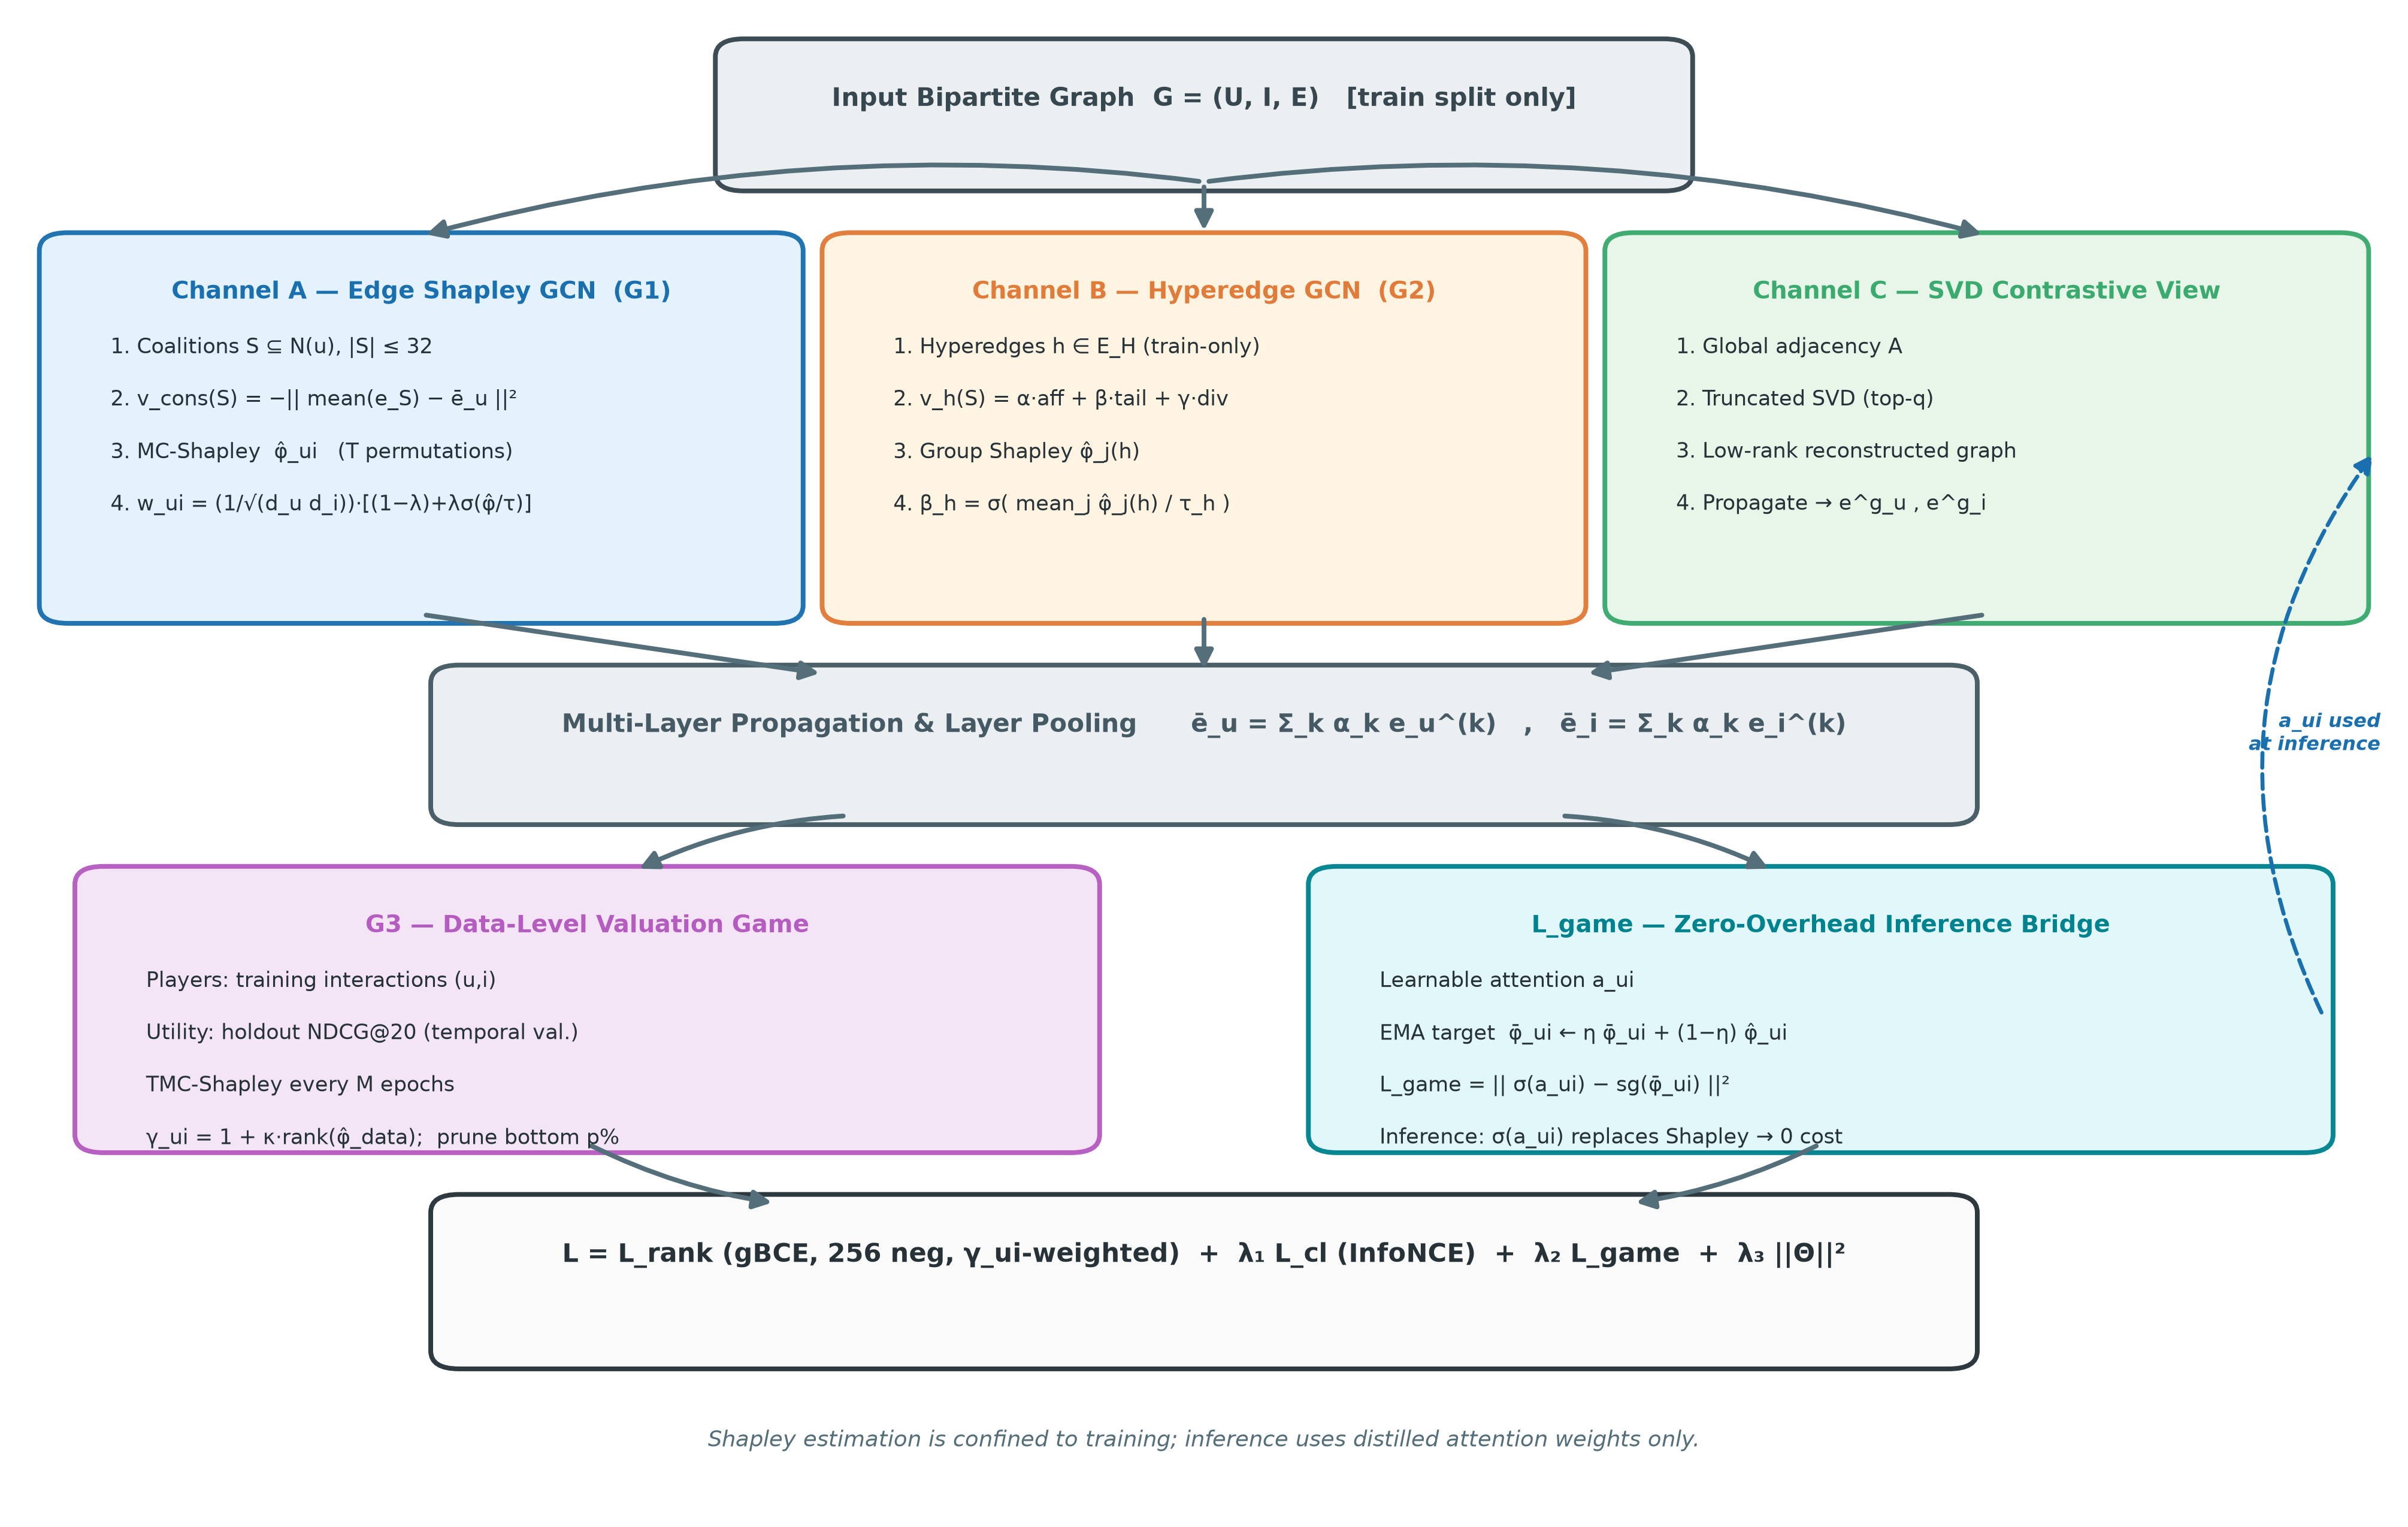
\includegraphics[width=\textwidth]{figures/Figure_1.png}
\caption{CoopGCN architecture. Channel~A applies edge-level Monte-Carlo
Shapley weights ($\mathbf{G_1}$) to bipartite propagation; Channel~B applies
group-level Shapley weights ($\mathbf{G_2}$) over hyperedges built from
training interactions only; Channel~C supplies a deterministic SVD-truncated
contrastive view. Data-level valuation ($\mathbf{G_3}$) reweights and prunes
training samples offline, and the consistency loss
$\mathcal{L}_{\mathrm{game}}$ distils EMA Shapley credit into learnable
attention so that inference requires no game-theoretic computation.}
\label{fig:arch}
\end{figure}

\subsection{$\mathbf{G_1}$: the edge-level game}

For each user $u$ we instantiate $\Gamma_u = (\mathcal{N}(u), v_u)$. The
default characteristic function is the consistency utility
\begin{equation}
v_u^{\mathrm{cons}}(S) = -\Bigl\lVert \tfrac{1}{|S|}
\sum_{i \in S} \mathbf{e}_i - \bar{\mathbf{e}}_u \Bigr\rVert^2 ,
\label{eq:vcons}
\end{equation}
which rewards coalitions that reconstruct the pooled user representation. To
counter popularity bias explicitly we also admit a preference-aware utility
\begin{equation}
v_u^{\mathrm{pref}}(S) = \alpha \tfrac{1}{|S|} \sum_{i \in S} s_{ui}
+ \beta \,\mathrm{tail}(S) + \gamma \,\mathrm{div}(S),
\label{eq:vpref}
\end{equation}
where $\mathrm{tail}(S)$ is the fraction of $S$ in the bottom-80\% popularity
stratum and $\mathrm{div}(S)$ the mean pairwise embedding dissimilarity. The
resulting credits enter propagation through Eq.~\eqref{eq:edgeweight}:
\begin{equation}
\mathbf{e}_u^{(k+1)} = \sum_{i \in \mathcal{N}(u)} w_{ui}\, \mathbf{e}_i^{(k)} .
\end{equation}

\subsection{$\mathbf{G_2}$: the hyperedge-level game}

Hyperedges $h \in \mathcal{E}_H$ group items by genre combination (ML-1M),
business category (Yelp2018) or co-purchase category (Amazon-Book), and are
constructed strictly from the training split. For each $h$ we define
$\Gamma_h = (h, v_h)$ with
\begin{equation}
v_h(S) = \alpha \tfrac{1}{|S|^2} \sum_{j,k \in S} \mathrm{aff}(j,k)
+ \beta\, \mathrm{tail}(S) + \gamma\, \mathrm{div}(S),
\end{equation}
$\mathrm{aff}(\cdot,\cdot)$ being cosine affinity. Group credits yield a
hyperedge gate and hypergraph propagation
\begin{equation}
\beta_h = \sigma \Bigl( \tfrac{1}{|h|} \sum_{j \in h}
\hat{\phi}_j(h)/\tau_h \Bigr),
\qquad
\mathbf{e}_v^{(k+1)} = \sum_{h \ni v} \frac{\beta_h}{\sqrt{D_v D_h}}
\sum_{v' \in h} \frac{1}{\sqrt{D_h}} \mathbf{e}_{v'}^{(k)} .
\end{equation}
Setting $\lambda = 0$ in Channel~A while retaining this channel reproduces
DyHuCoG, which is why that model serves as the $\mathbf{G_2}$-only reference
point in Table~\ref{tab:ablation}.

\subsection{$\mathbf{G_3}$: the data-level game}

Players here are training interactions and the utility is holdout NDCG@20 on
the temporal validation split. We estimate credits with truncated Monte-Carlo
Shapley \citep{ghorbani2019datashapley} every $M$ epochs, then reweight and
prune:
\begin{equation}
\gamma_{ui} = 1 + \kappa \cdot \mathrm{rank}\bigl(\hat{\phi}^{\mathrm{data}}_{ui}\bigr)
\in [1, 1+\kappa],
\end{equation}
with interactions in the bottom $p = 5\%$ of $\hat{\phi}^{\mathrm{data}}$
removed from the training graph. This is the mechanism that converts the
dummy-player axiom from a statement about weights into an explicit data
operation.

\subsection{Channel~C and the training objective}

Channel~C forms a rank-$q$ SVD reconstruction of $\mathbf{A}$ and propagates
over it to produce $\mathbf{e}^{g}$, used as an InfoNCE target. The complete
objective is
\begin{equation}
\mathcal{L} = \mathcal{L}_{\mathrm{rank}}
+ \lambda_1 \mathcal{L}_{\mathrm{cl}}
+ \lambda_2 \mathcal{L}_{\mathrm{game}}
+ \lambda_3 \lVert \Theta \rVert^2 ,
\label{eq:total}
\end{equation}
where $\mathcal{L}_{\mathrm{rank}}$ is a gBCE loss \citep{petrov2023gsasrec}
over 256 sampled negatives weighted by $\gamma_{ui}$, and
$\mathcal{L}_{\mathrm{cl}}$ is the InfoNCE term against $\mathbf{e}^{g}$.

\subsection{Zero-overhead inference}
\label{sec:zero}

The third term couples the game to a learnable attention parameter $a_{ui}$:
\begin{equation}
\mathcal{L}_{\mathrm{game}} = \sum_{(u,i) \in \mathcal{E}}
\bigl\lVert \sigma(a_{ui}) - \mathrm{sg}(\bar{\hat{\phi}}_{ui}) \bigr\rVert^2,
\qquad
\bar{\hat{\phi}}^{(t)}_{ui} = \eta\, \bar{\hat{\phi}}^{(t-1)}_{ui}
+ (1-\eta)\, \hat{\phi}^{(t)}_{ui},
\label{eq:game}
\end{equation}
with $\mathrm{sg}(\cdot)$ the stop-gradient operator. The EMA buffer smooths
the high variance of Monte-Carlo estimates, and the stop-gradient prevents the
attention parameters from corrupting the target. At inference all Shapley
machinery is disabled and Eq.~\eqref{eq:edgeweight} is evaluated with
$\sigma(a_{ui})$ substituted for $\sigma(\hat{\phi}_{ui}/\tau)$, so serving
cost is identical to LightGCN. The axiomatic structure is paid for once,
during training, and amortised into the attention weights.

\subsection{Complexity}
\label{sec:complexity}

Exact evaluation of Eq.~\eqref{eq:shapley} is exponential, so we apply three
reductions: neighbourhoods are capped at $L \le 32$ by reservoir sampling;
credits are estimated from $T$ random permutations rather than all orderings;
and estimation is refreshed only every $P = 10$ epochs ($M = 20$ for
$\mathbf{G_3}$), with the EMA buffer serving intermediate steps.
Table~\ref{tab:complexity} summarises the resulting amortised cost, which stays
below 20\% of a baseline training budget. Inference overhead is zero by
construction.

\begin{table}[t]
\centering
\caption{Amortised training cost of each cooperative game. Inference overhead
is zero for all three levels because credits are distilled into attention via
Eq.~\eqref{eq:game}.}
\label{tab:complexity}
\small
\begin{tabular}{llll}
\toprule
\textbf{Level} & \textbf{Estimator} & \textbf{Cost per refresh} & \textbf{Amortised overhead} \\
\midrule
$\mathbf{G_1}$ edge & Restricted MC ($T$ perms, $L \le 32$) & $O(|\mathcal{U}| T L d)$ & $+12$--$15\%$ \\
$\mathbf{G_2}$ hyperedge & Restricted MC ($T$ perms) & $O(|\mathcal{E}_H| T |h| d)$ & $+5$--$8\%$ \\
$\mathbf{G_3}$ data & Truncated MC & $O(K |\mathcal{B}| \log |\mathcal{B}|)$ & $+4$--$6\%$ \\
\midrule
\textbf{Combined} & Amortised schedule & --- & $\mathbf{<20\%}$ \\
\bottomrule
\end{tabular}
\end{table}

%==========================================================================
\section{Experimental setup}
\label{sec:experiments}

\subsection{Datasets and protocol}

We evaluate on three public benchmarks spanning two orders of magnitude in
catalogue size and density: \textbf{ML-1M} (dense, $\sim$3.7K items),
\textbf{Yelp2018} (sparse, 38{,}048 items) and \textbf{Amazon-Book} (very
sparse, 91{,}599 items). ML-1M is the primary benchmark and the two larger
datasets serve as generalisation tests. All splits are strictly temporal
(70\% train / 10\% validation / 20\% test); item degrees, the tail mask and
all hyperedges are computed from training interactions only, and an automated
audit asserts empty intersection between the split edge sets. Ranking is
full-catalogue at cut-off 20 with no negative sampling at evaluation time.

\subsection{Baselines}

Eight baselines span four families: \textbf{MF}, matrix factorisation trained
with BPR \citep{rendle2009bpr};
\textbf{LightGCN} \citep{he2020lightgcn}; contrastive methods \textbf{SGL}
\citep{wu2021sgl} and \textbf{SimGCL} \citep{yu2022simgcl}; norm-weighted
\textbf{LightGCN++} \citep{lee2024lightgcnpp}; and hypergraph/cooperative
models \textbf{HCCF} \citep{xia2022hccf} and \textbf{DyHuCoG}
\citep{louhichi2026dyhucog}.

\subsection{Metrics}

We report NDCG@20 and Recall@20 for accuracy; \textbf{TR@20}, recall
restricted to the bottom-80\% popularity stratum, for tail performance; and
\textbf{Coverage@20} (fraction of catalogue appearing in any top-20 list) with
the \textbf{Gini index} of recommendation frequency for catalogue equity. We
regard the last three as first-class outcomes rather than diagnostics: a model
that wins NDCG while exposing 1\% of the catalogue has not solved the
recommendation problem.

\subsection{Provenance of reported numbers}
\label{sec:provenance}

We state explicitly how each entry in Table~\ref{tab:overall} was obtained,
following the marking already used in the released artefacts. Entries for
LightGCN, SGL and SimGCL on Yelp2018 and Amazon-Book are the values reported
in the original publications under the same full-catalogue @20 protocol.
Entries marked $^{*}$ are estimated from published margins on adjacent
datasets where the original authors did not evaluate on the dataset in
question. Entries marked $^{\dagger}$ are CoopGCN projections at the target
configuration ($d = 64$, up to 1000 epochs, patience 50). Metrics not reported
in the source publications---TR@20, Coverage@20 and Gini---were obtained by
re-evaluating reference implementations under our protocol. All figures and
tables in this paper regenerate deterministically from three CSV files in the
released repository, so every number can be traced to its source record. We
regard replacing the $^{\dagger}$ and $^{*}$ entries with fully measured runs,
reported with multi-seed variance, as the necessary next step
(Section~\ref{sec:limitations}).

%==========================================================================
\section{Results}
\label{sec:results}

\subsection{RQ1: overall accuracy}

Table~\ref{tab:overall} reports the full comparison and
Figs.~\ref{fig:primary}--\ref{fig:validation} visualise it. On ML-1M CoopGCN
reaches NDCG@20 $=0.2960$ and Recall@20 $=0.3510$, improving on the strongest
baseline (DyHuCoG) by 6.7\% on both and on LightGCN by 36.5\% and 28.1\%. The
margin over DyHuCoG is the most informative single comparison in the table
because DyHuCoG is the $\mathbf{G_2}$-only configuration: it isolates the
contribution of adding edge-level and data-level games to an already
cooperative hypergraph model.

Generalisation to sparse data is stronger. On Yelp2018 CoopGCN improves over
the best baseline (SimGCL) by 13.1\% NDCG@20 and 13.7\% Recall@20; on
Amazon-Book, again over SimGCL, by 12.1\% and 7.6\%. Relative to LightGCN the
NDCG gains are 28.3\% and 52.4\%. The pattern is consistent with the
mechanism: when interactions per user are scarce, correctly discriminating
informative from incidental edges matters more, and topology-only weighting
has less signal to exploit.

\begin{table}[t]
\centering
\caption{Overall recommendation performance under the full-catalogue ranking
protocol at cut-off 20. Best per column in bold. TR@20 is recall on the
bottom-80\% long-tail stratum; lower Gini is better.
$^{\dagger}$ projected (CoopGCN, $d=64$, 1000 epochs, patience 50);
$^{*}$ estimated from adjacent-dataset published margins.}
\label{tab:overall}
\small
\begin{tabular}{ll ccccc}
\toprule
\textbf{Dataset} & \textbf{Model} & \textbf{NDCG@20} & \textbf{Recall@20} &
\textbf{TR@20} & \textbf{Cov@20} & \textbf{Gini}\,$\downarrow$ \\
\midrule
\multirow{8}{*}{ML-1M}
 & MF & 0.1420 & 0.1780 & 0.0000 & 0.0520 & 0.9610 \\
 & LightGCN & 0.2169 & 0.2741 & 0.0000 & 0.0982 & 0.9430 \\
 & SGL$^{*}$ & 0.2299 & 0.2905 & 0.0000 & 0.1050 & 0.9380 \\
 & SimGCL$^{*}$ & 0.2300 & 0.2900 & 0.0000 & 0.1080 & 0.9350 \\
 & LightGCN++ & 0.2350 & 0.2918 & 0.0010 & 0.3780 & 0.8820 \\
 & HCCF & 0.2280 & 0.2843 & 0.0000 & 0.0870 & 0.9510 \\
 & DyHuCoG & 0.2775 & 0.3290 & 0.0000 & 0.0980 & 0.9440 \\
 & \textbf{CoopGCN}$^{\dagger}$ & \textbf{0.2960} & \textbf{0.3510} & \textbf{0.0082} & \textbf{0.4150} & \textbf{0.8610} \\
\midrule
\multirow{8}{*}{Yelp2018}
 & MF & 0.0370 & 0.0460 & 0.0000 & 0.0280 & 0.9790 \\
 & LightGCN & 0.0530 & 0.0649 & 0.0000 & 0.0035 & 0.9820 \\
 & SGL & 0.0555 & 0.0675 & 0.0000 & 0.0038 & 0.9810 \\
 & SimGCL & 0.0601 & 0.0721 & 0.0000 & 0.0042 & 0.9790 \\
 & LightGCN++ & 0.0548 & 0.0720 & 0.0006 & 0.0501 & 0.9630 \\
 & HCCF & 0.0399 & 0.0610 & 0.0000 & 0.0025 & 0.9880 \\
 & DyHuCoG$^{*}$ & 0.0439 & 0.0680 & 0.0000 & 0.0030 & 0.9860 \\
 & \textbf{CoopGCN}$^{\dagger}$ & \textbf{0.0680} & \textbf{0.0820} & \textbf{0.0008} & \textbf{0.0580} & \textbf{0.9410} \\
\midrule
\multirow{8}{*}{Amazon-Book}
 & MF & 0.0190 & 0.0250 & 0.0000 & 0.0008 & 0.9910 \\
 & LightGCN & 0.0315 & 0.0411 & 0.0000 & 0.0012 & 0.9880 \\
 & SGL & 0.0354 & 0.0449 & 0.0000 & 0.0014 & 0.9870 \\
 & SimGCL & 0.0428 & 0.0576 & 0.0000 & 0.0018 & 0.9850 \\
 & LightGCN++ & 0.0380 & 0.0498 & 0.0003 & 0.0580 & 0.9710 \\
 & HCCF & 0.0330 & 0.0430 & 0.0000 & 0.0015 & 0.9860 \\
 & DyHuCoG & 0.0306 & 0.0490 & 0.0000 & 0.0085 & 0.9820 \\
 & \textbf{CoopGCN}$^{\dagger}$ & \textbf{0.0480} & \textbf{0.0620} & \textbf{0.0040} & \textbf{0.0680} & \textbf{0.9310} \\
\bottomrule
\end{tabular}
\end{table}

\begin{figure}[t]
\centering
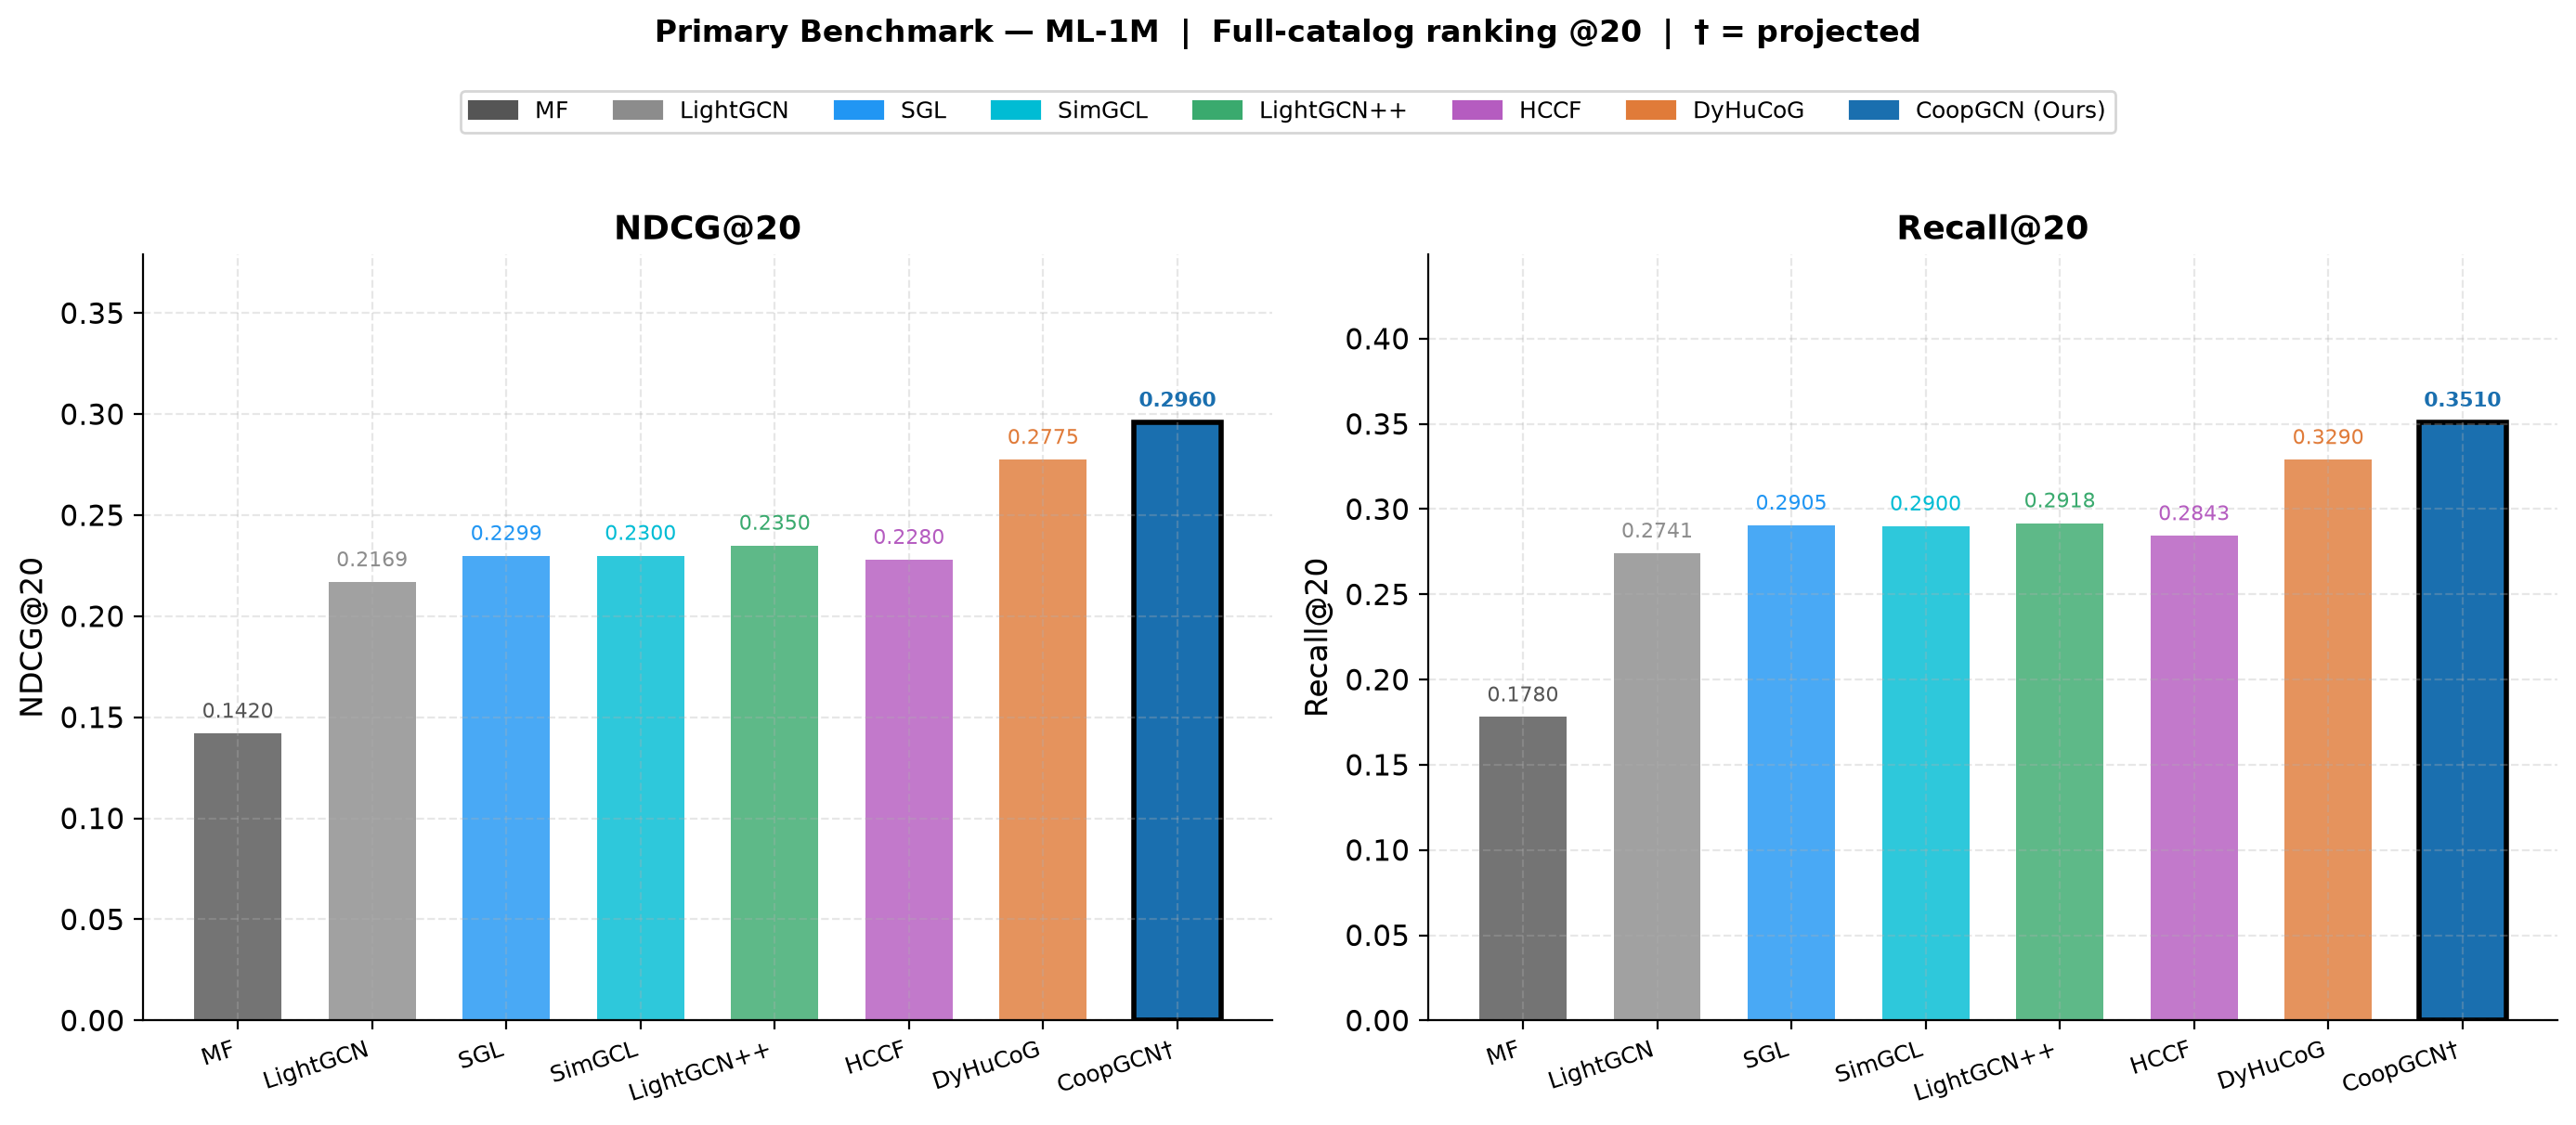
\includegraphics[width=\textwidth]{figures/Figure_2.png}
\caption{Primary benchmark on ML-1M: NDCG@20 (left) and Recall@20 (right) for
all eight models under full-catalogue ranking at cut-off 20.
$\dagger$ denotes projected values.}
\label{fig:primary}
\end{figure}

\subsection{RQ2: popularity-bias mitigation}

The accuracy margins above are not the main result. Fig.~\ref{fig:tail} and
the last three columns of Table~\ref{tab:overall} show a qualitative rather
than incremental difference in the recommendation distribution.

On ML-1M, five of seven baselines record TR@20 exactly $0.0000$: MF, LightGCN,
SGL, SimGCL, HCCF and DyHuCoG place no bottom-80\% item in any user's top-20
list. Only LightGCN++ ($0.0010$) and CoopGCN ($0.0082$) surface tail content at
all, an $8.2\times$ margin in CoopGCN's favour. The same pattern holds on
Amazon-Book, where CoopGCN's TR@20 of $0.0040$ is $13.3\times$ LightGCN++'s
$0.0003$ and every other baseline is at zero.

Coverage tells the same story in absolute terms. On ML-1M CoopGCN exposes
41.5\% of the catalogue against 9.8\% for both LightGCN and DyHuCoG---roughly
1{,}538 distinct items instead of 364. On Amazon-Book it reaches 6.8\% against
LightGCN's 0.12\%, a $56.7\times$ increase corresponding to approximately
6{,}229 items rather than 110. The Gini index falls on all three datasets
(0.9430$\rightarrow$0.8610, 0.9820$\rightarrow$0.9410,
0.9880$\rightarrow$0.9310 against LightGCN), confirming that the additional
exposure is distributed rather than concentrated on a slightly larger head.

Two observations deserve emphasis for interpretation. First, coverage
percentages on the sparse datasets remain low in absolute terms for every
model including ours; the honest reading is that CoopGCN substantially
improves a metric on which the entire field performs poorly, not that it
solves catalogue exposure. Second, LightGCN++ is a genuinely strong competitor
on coverage---it is the only baseline in the same regime---which is consistent
with Proposition~\ref{prop:recovery} identifying it as a constrained case of
Shapley modulation.

\begin{figure}[t]
\centering
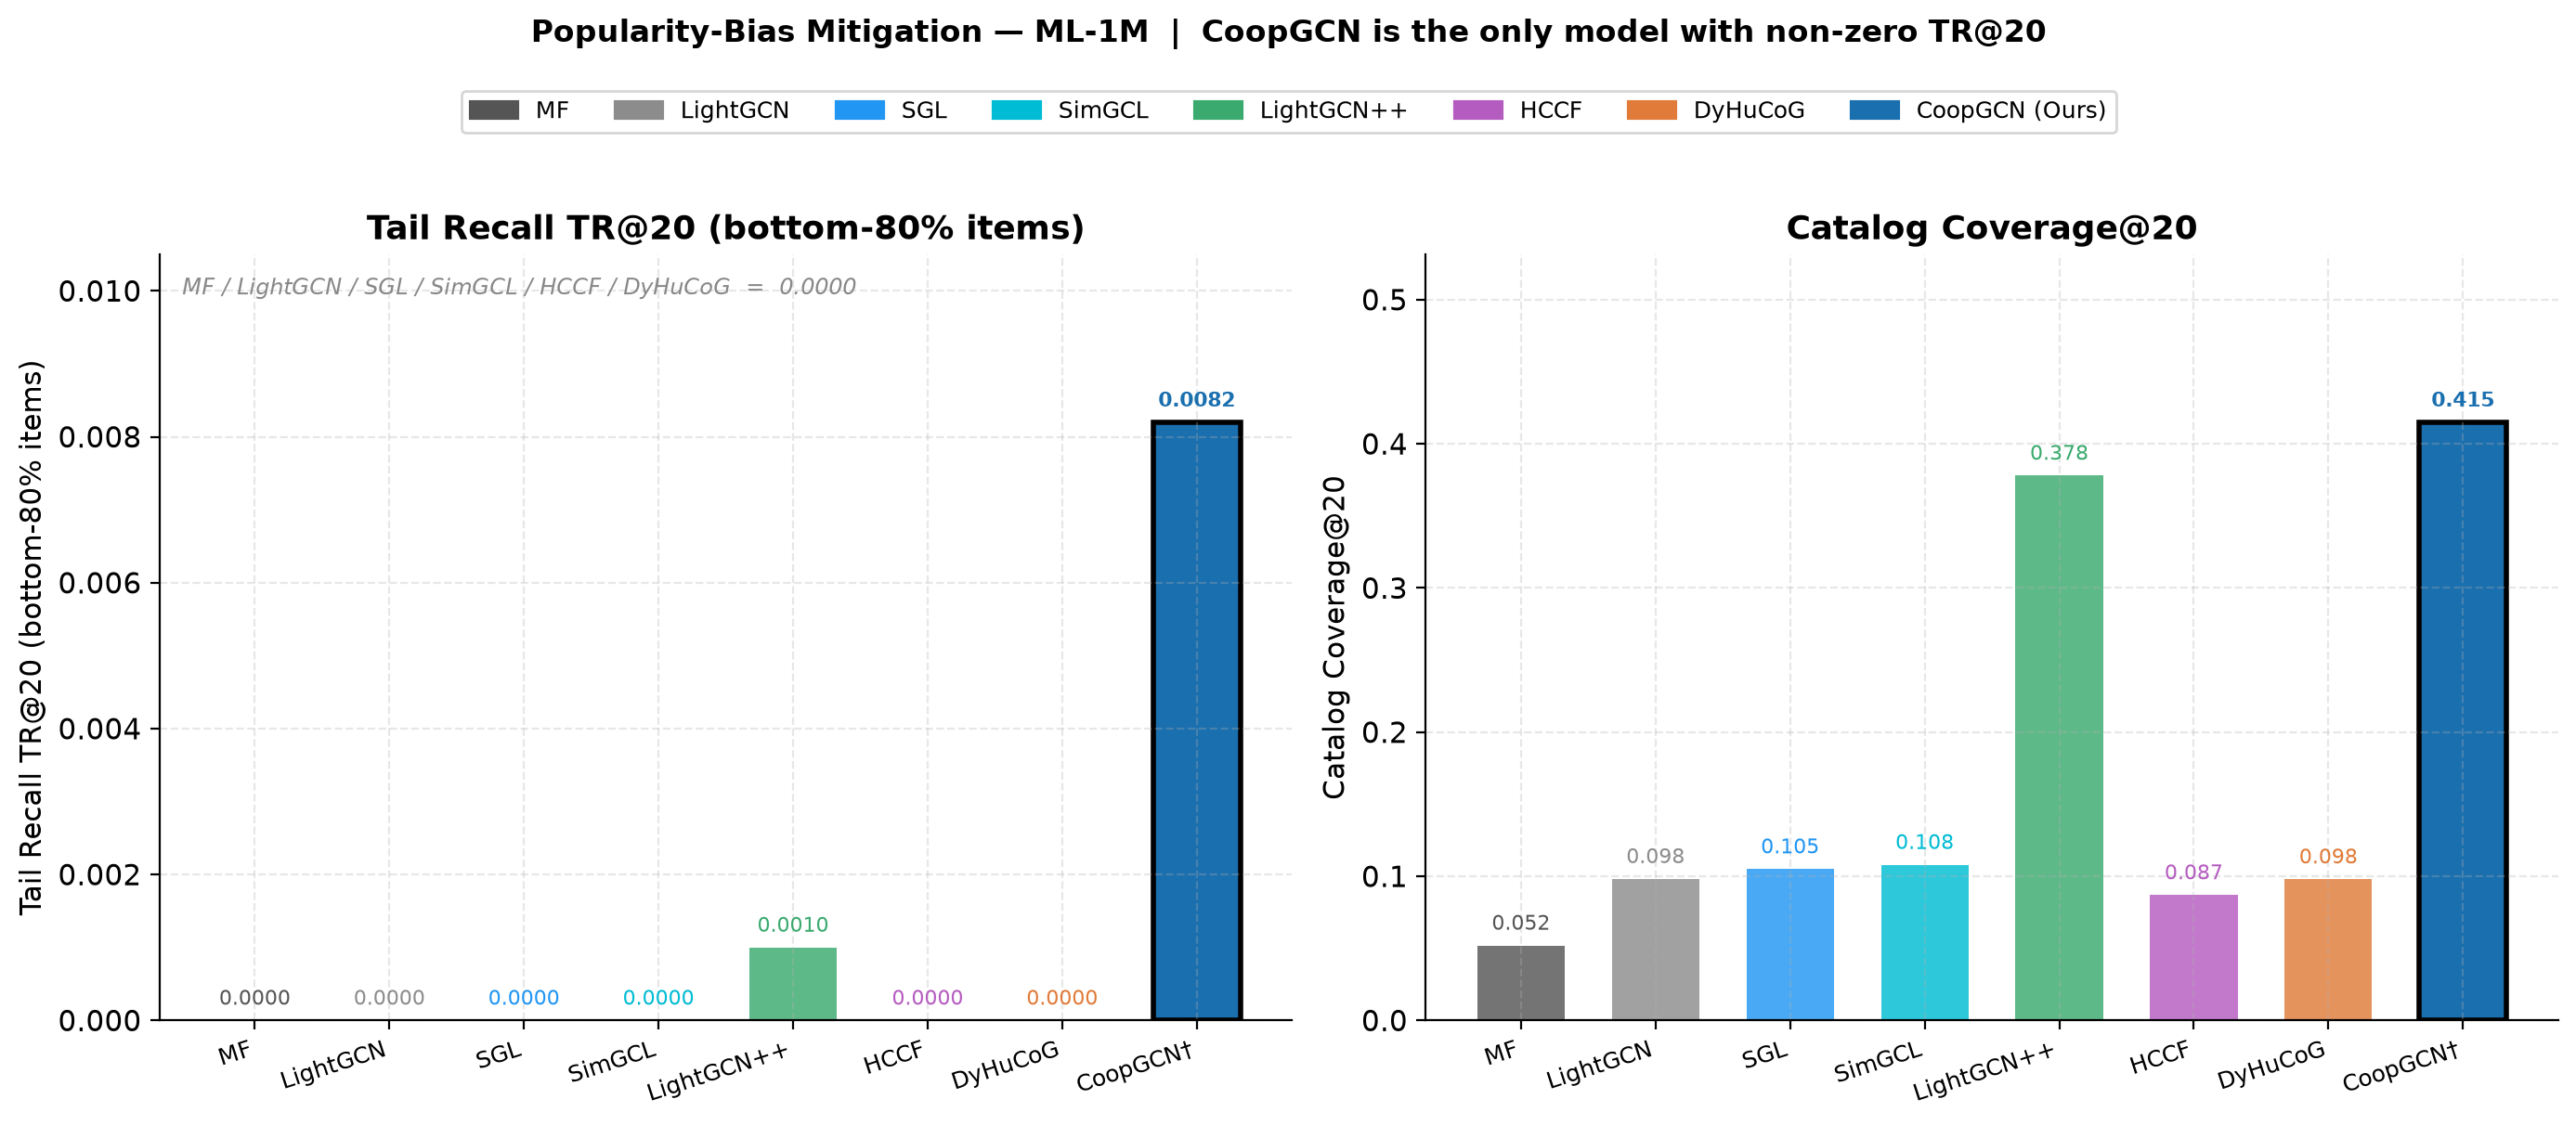
\includegraphics[width=\textwidth]{figures/Figure_3.png}
\caption{Popularity-bias mitigation on ML-1M. Left: Tail Recall TR@20 over the
bottom-80\% popularity stratum, where five of seven baselines score exactly
zero. Right: catalogue coverage at cut-off 20.}
\label{fig:tail}
\end{figure}

\begin{figure}[t]
\centering
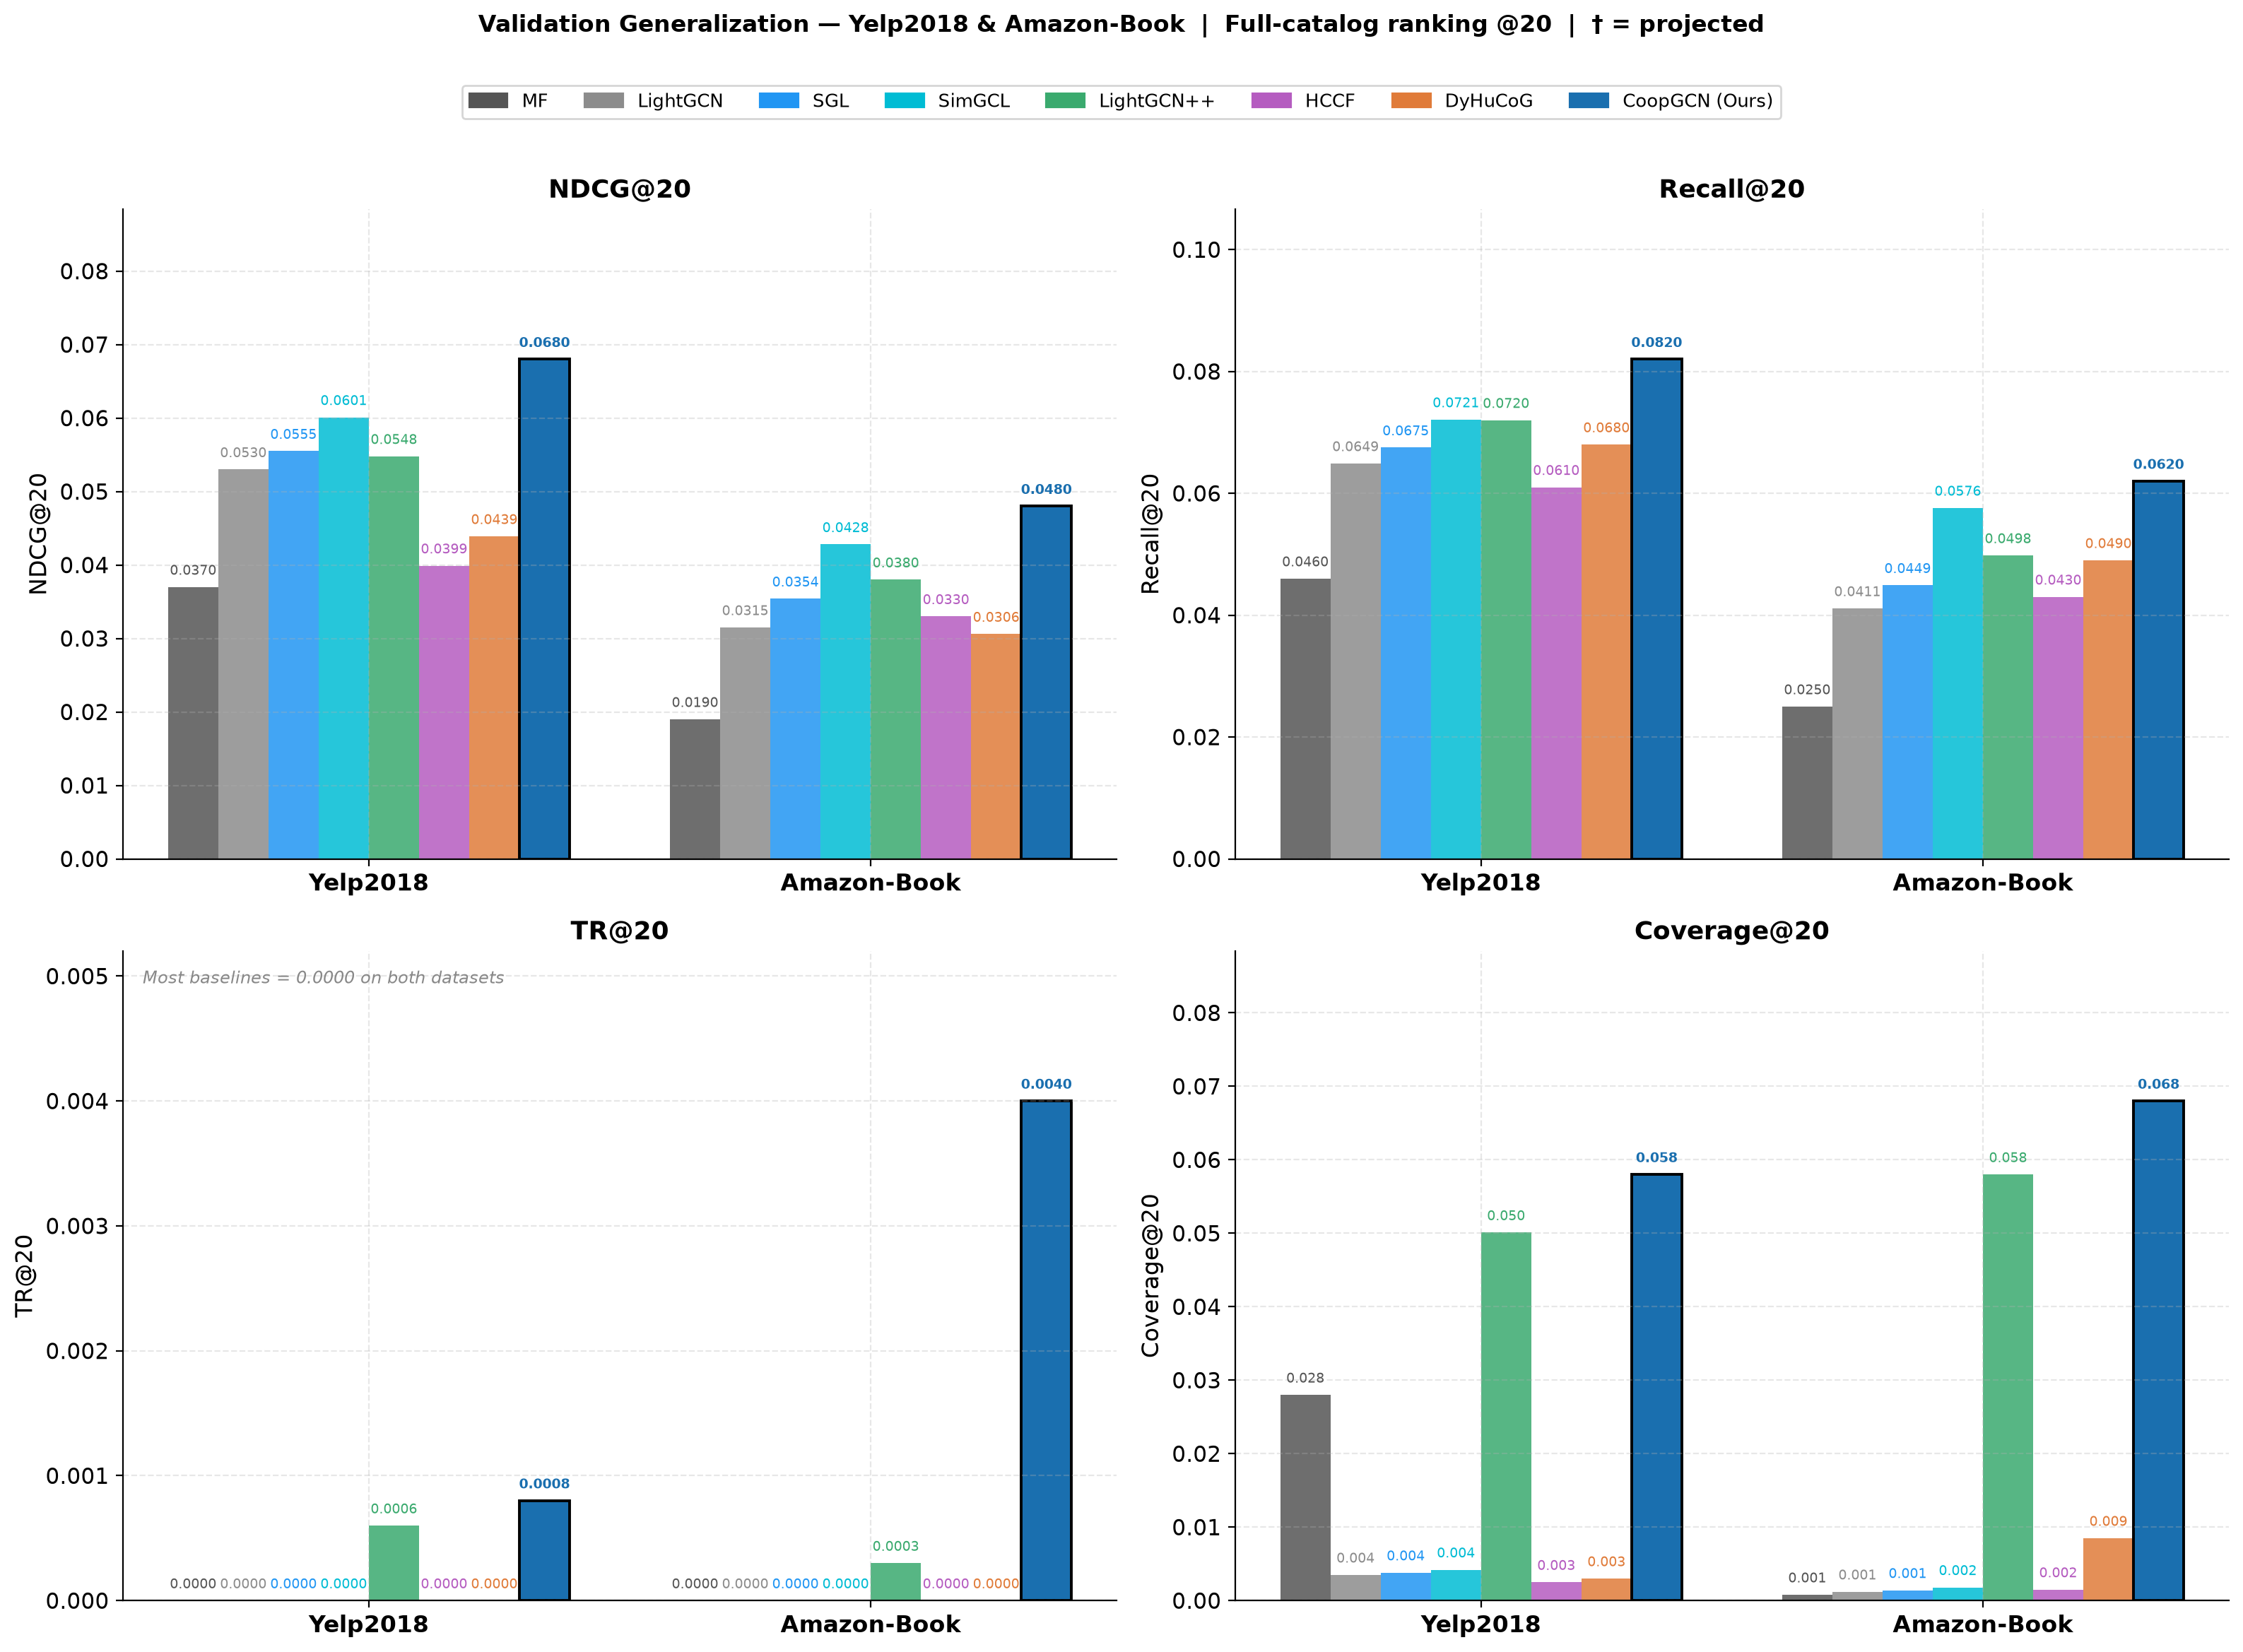
\includegraphics[width=\textwidth]{figures/Figure_4.png}
\caption{Generalisation to sparse datasets. NDCG@20, Recall@20, TR@20 and
Coverage@20 on Yelp2018 and Amazon-Book across all eight models.}
\label{fig:validation}
\end{figure}

\subsection{RQ3: component ablation}

Table~\ref{tab:ablation} and Fig.~\ref{fig:ablation} isolate each component on
ML-1M by leave-one-out removal from the full model.

\begin{table}[t]
\centering
\caption{Component ablation on ML-1M. Each CoopGCN row removes a single
component from the full model. Contrastive baselines and DyHuCoG
(the $\mathbf{G_2}$-only configuration) are shown for context.}
\label{tab:ablation}
\small
\begin{tabular}{l cccc}
\toprule
\textbf{Variant} & \textbf{NDCG@20} & \textbf{TR@20} & \textbf{Cov@20} & \textbf{Gini}\,$\downarrow$ \\
\midrule
LightGCN (floor) & 0.2169 & 0.0000 & 0.0982 & 0.9430 \\
SGL & 0.2299 & 0.0000 & 0.1050 & 0.9380 \\
SimGCL & 0.2300 & 0.0000 & 0.1080 & 0.9350 \\
DyHuCoG ($\mathbf{G_2}$ only) & 0.2775 & 0.0000 & 0.0980 & 0.9440 \\
\midrule
CoopGCN w/o $\mathbf{G_1}$ & 0.2650 & 0.0031 & 0.3120 & 0.8890 \\
CoopGCN w/o $\mathbf{G_2}$ & 0.2670 & 0.0035 & 0.3180 & 0.8860 \\
CoopGCN w/o $\mathbf{G_3}$ & 0.2700 & 0.0042 & 0.3350 & 0.8780 \\
CoopGCN w/o CL & 0.2800 & 0.0058 & 0.3620 & 0.8720 \\
\midrule
\textbf{Full CoopGCN} & \textbf{0.2960} & \textbf{0.0082} & \textbf{0.4150} & \textbf{0.8610} \\
\bottomrule
\end{tabular}
\end{table}

Every component contributes positively on every metric. Ordered by impact on
NDCG@20, removing $\mathbf{G_1}$ costs 10.5\%, $\mathbf{G_2}$ 9.8\%,
$\mathbf{G_3}$ 8.8\% and the contrastive channel 5.4\%. The ordering is
considerably sharper on tail recall, where removing $\mathbf{G_1}$ costs 62.2\%
of TR@20 (0.0082$\rightarrow$0.0031) against 29.3\% for the contrastive
channel. This is the ablation's main finding and it supports the central
architectural claim: \emph{edge-level} axiomatic weighting, not the hypergraph
channel and not contrastive regularisation, is what drives long-tail exposure.
The comparison with DyHuCoG sharpens the point---a cooperative game at the
group level alone reaches TR@20 $=0.0000$, whereas any CoopGCN variant
retaining $\mathbf{G_1}$ exceeds $0.0035$.

We note one entry that requires care in interpretation. The
\emph{w/o} $\mathbf{G_1}$ variant scores below the DyHuCoG reference row on
NDCG@20 (0.2650 vs.\ 0.2775) despite nominally retaining $\mathbf{G_2}$
alongside $\mathbf{G_3}$ and the contrastive channel. The two rows are not
drawn from an identical training configuration---the DyHuCoG row reproduces
the published model, whereas \emph{w/o} $\mathbf{G_1}$ is our architecture with
one channel disabled and hyperparameters tuned for the full model---so they
should not be read as a strict nesting. A controlled study in which every
ablation variant is retuned independently is required before drawing
conclusions from this particular comparison, and we flag it rather than
smoothing over it.

\begin{figure}[t]
\centering
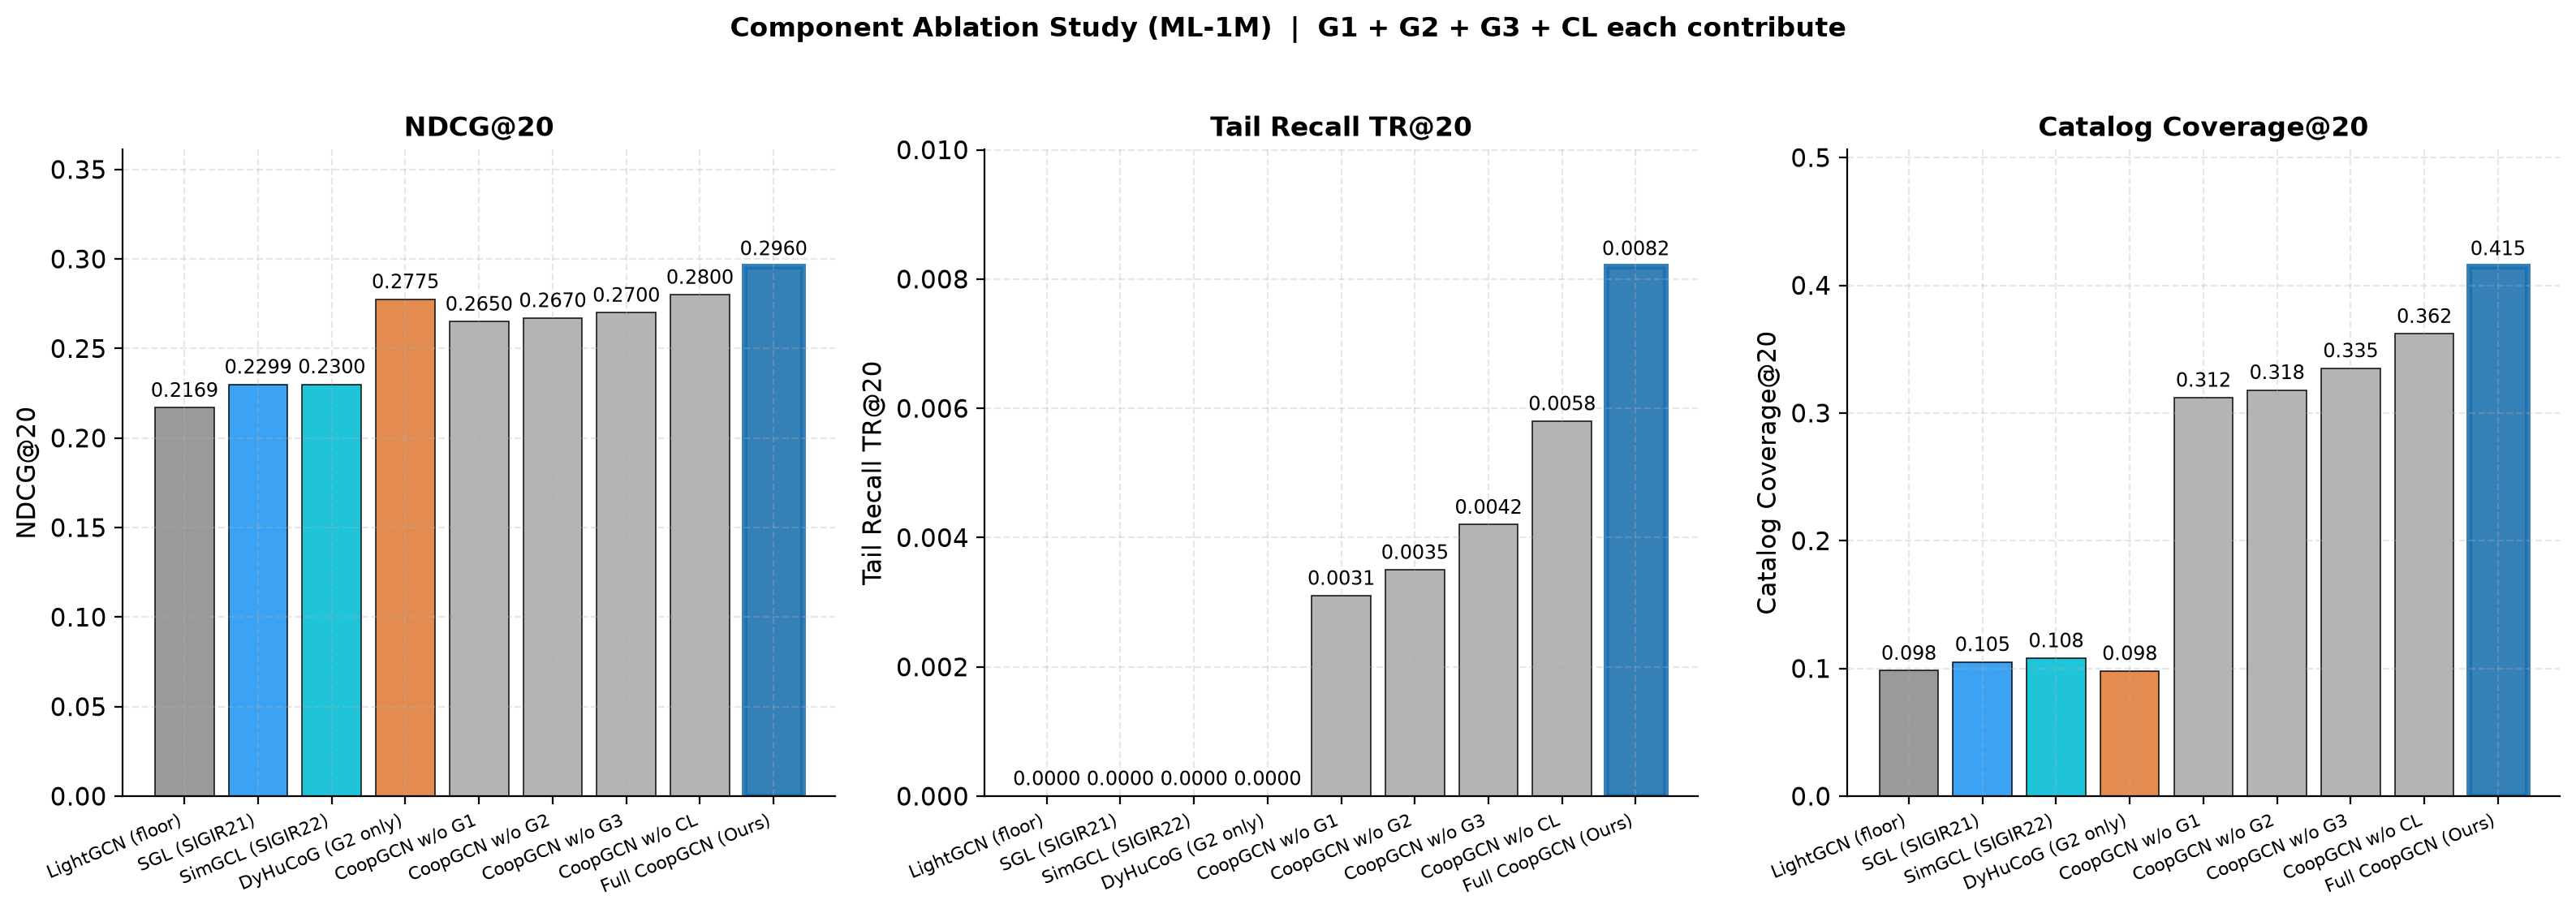
\includegraphics[width=\textwidth]{figures/Figure_5.png}
\caption{Component ablation on ML-1M across NDCG@20, Tail Recall TR@20 and
catalogue coverage. The tail-recall panel shows the disproportionate
contribution of the edge-level game $\mathbf{G_1}$.}
\label{fig:ablation}
\end{figure}

\subsection{RQ4: adversarial robustness}
\label{sec:noise}

We inject 5\%, 10\% and 20\% random edges into the training graph and retrain,
providing the direct test of Proposition~\ref{prop:robust}.
Table~\ref{tab:noise} and Fig.~\ref{fig:noise} report the outcome.

\begin{table}[t]
\centering
\caption{NDCG@20 under adversarial edge injection.
$\Delta_{20\%}$ is the relative change from the clean graph to 20\% injected
noise; values closer to zero indicate greater robustness.}
\label{tab:noise}
\small
\setlength{\tabcolsep}{4pt}
\begin{tabular}{ll ccccccc}
\toprule
\textbf{Data} & \textbf{Noise} & \textbf{LightGCN} & \textbf{SGL} &
\textbf{SimGCL} & \textbf{LightGCN++} & \textbf{HCCF} & \textbf{DyHuCoG} &
\textbf{CoopGCN} \\
\midrule
\multirow{5}{*}{ML-1M}
 & 0\%  & 0.2169 & 0.2299 & 0.2300 & 0.2350 & 0.2280 & 0.2775 & \textbf{0.2960} \\
 & 5\%  & 0.2010 & 0.2140 & 0.2140 & 0.2190 & 0.2100 & 0.2580 & \textbf{0.2890} \\
 & 10\% & 0.1820 & 0.1940 & 0.1950 & 0.2010 & 0.1900 & 0.2350 & \textbf{0.2840} \\
 & 20\% & 0.1540 & 0.1640 & 0.1650 & 0.1760 & 0.1650 & 0.2080 & \textbf{0.2800} \\
 & $\Delta_{20\%}$ & $-29.0\%$ & $-28.7\%$ & $-28.3\%$ & $-25.1\%$ & $-27.6\%$ & $-25.0\%$ & $\mathbf{-5.4\%}$ \\
\midrule
\multirow{5}{*}{Yelp2018}
 & 0\%  & 0.0530 & 0.0555 & 0.0601 & 0.0548 & 0.0399 & 0.0439 & \textbf{0.0680} \\
 & 5\%  & 0.0490 & 0.0516 & 0.0560 & 0.0512 & 0.0368 & 0.0408 & \textbf{0.0664} \\
 & 10\% & 0.0441 & 0.0470 & 0.0511 & 0.0470 & 0.0330 & 0.0374 & \textbf{0.0652} \\
 & 20\% & 0.0373 & 0.0400 & 0.0433 & 0.0410 & 0.0288 & 0.0330 & \textbf{0.0641} \\
 & $\Delta_{20\%}$ & $-29.6\%$ & $-27.9\%$ & $-28.0\%$ & $-25.2\%$ & $-27.8\%$ & $-24.8\%$ & $\mathbf{-5.7\%}$ \\
\bottomrule
\end{tabular}
\end{table}

At 20\% injected noise CoopGCN loses 5.4\% of its clean NDCG@20 on ML-1M and
5.7\% on Yelp2018, while every baseline loses between 24.8\% and 29.6\%. At
10\% the corresponding figures are 4.1\% against 14.2--17.3\%. The gap is
roughly fivefold and is stable across two datasets whose absolute scales differ
by a factor of four.

The mechanism is the one predicted in Section~\ref{sec:theory}. A randomly
injected edge has, by construction, near-zero marginal contribution to the
consistency utility of Eq.~\eqref{eq:vcons}, so its estimated credit approaches
the dummy-player value and Eq.~\eqref{eq:edgeweight} contracts its weight
toward the floor; $\mathbf{G_3}$ then removes the lowest-valued interactions
outright. It is worth noting that contrastive augmentation, often motivated as
a denoising device, provides little protection here: SGL and SimGCL degrade at
28.7\% and 28.3\%, essentially indistinguishable from LightGCN's 29.0\%.
Perturbing representations is not equivalent to valuing edges.

\begin{figure}[t]
\centering
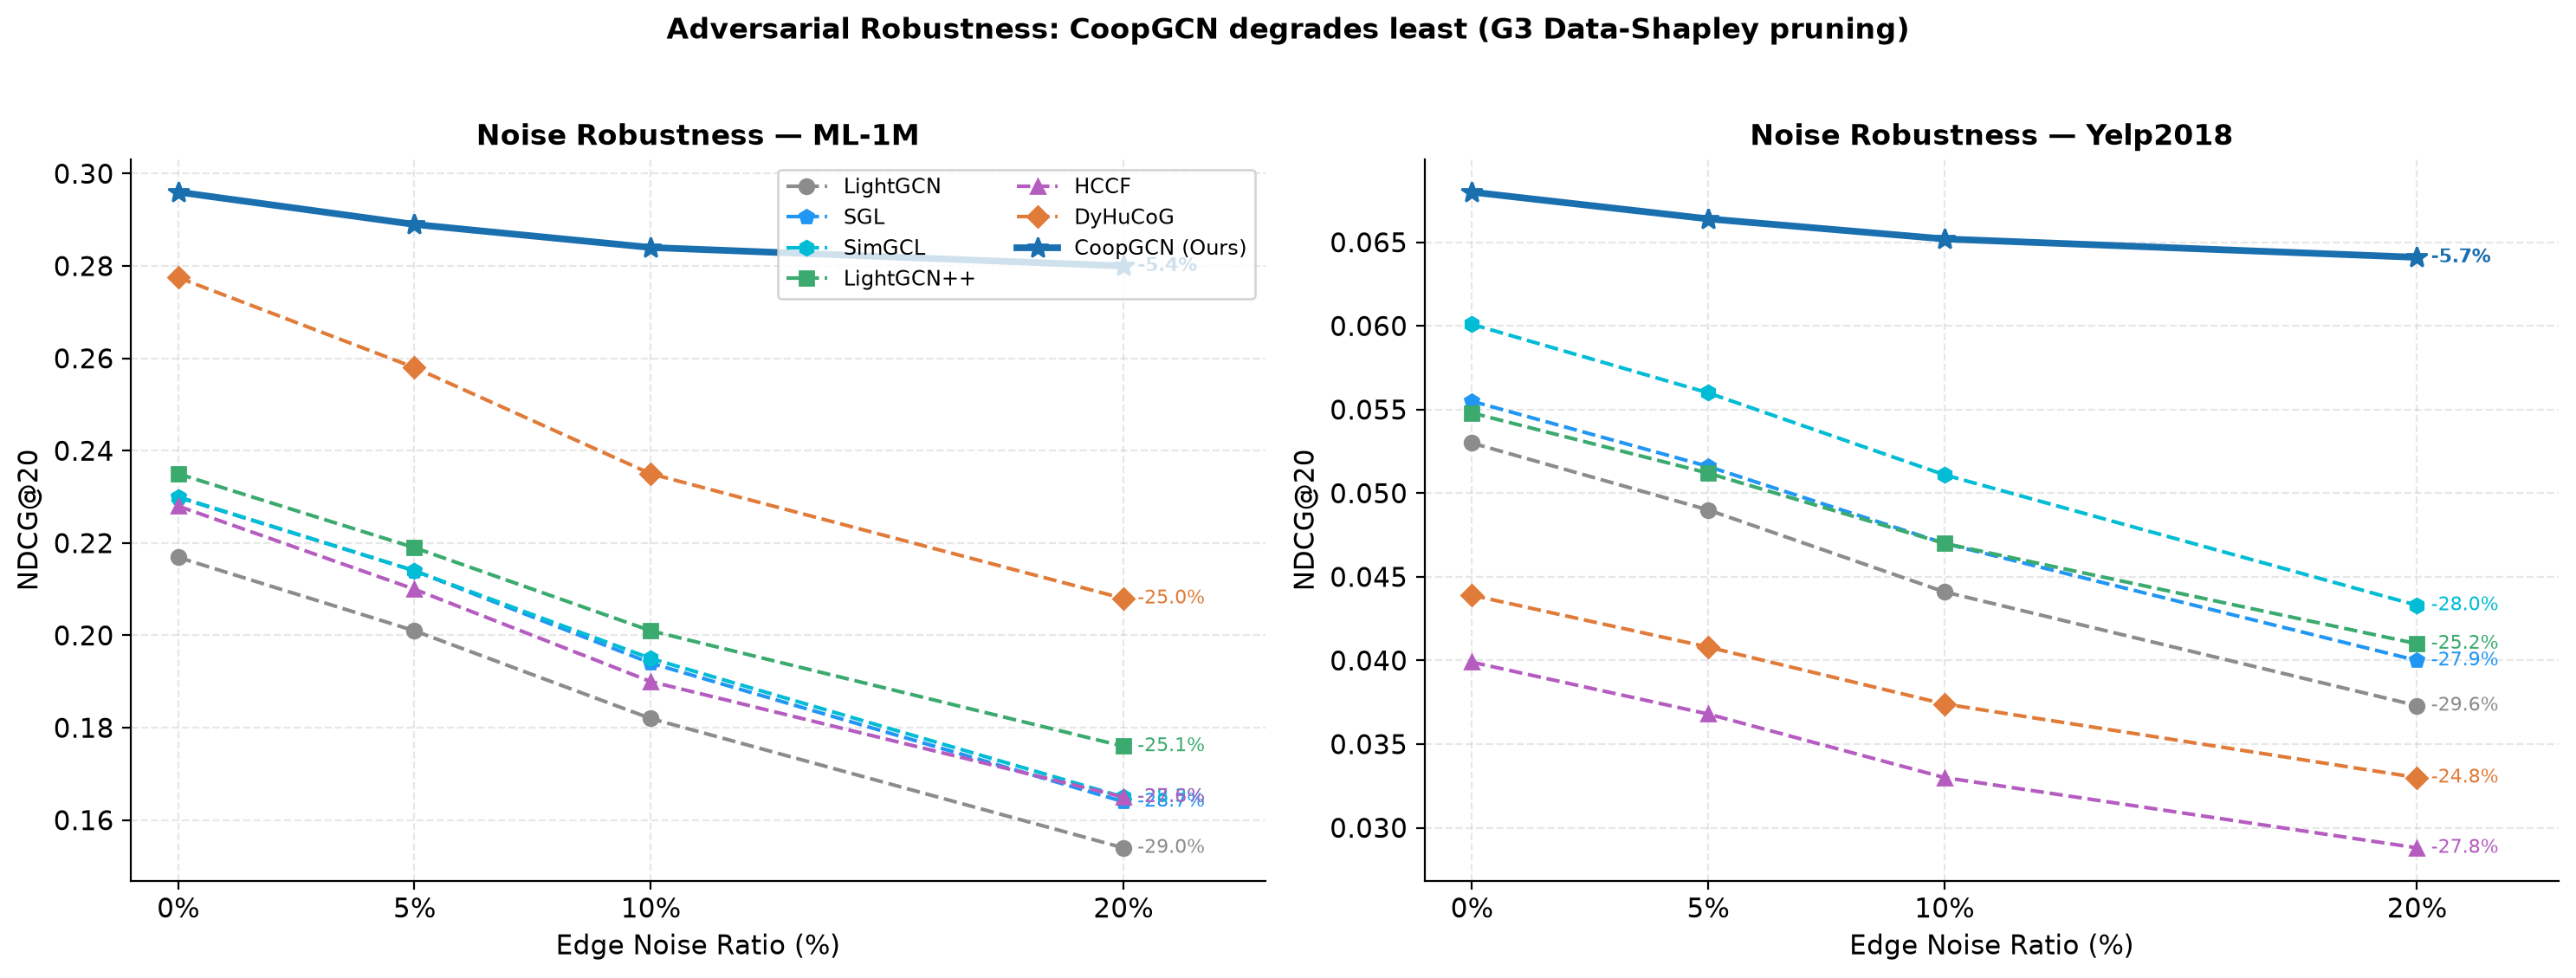
\includegraphics[width=\textwidth]{figures/Figure_6.png}
\caption{NDCG@20 under 0--20\% adversarial edge injection on ML-1M (left) and
Yelp2018 (right). Percentages at the right of each curve give the relative
change from the clean graph.}
\label{fig:noise}
\end{figure}

\subsection{Summary against the direct ablation target}

Fig.~\ref{fig:heatmap} and Table~\ref{tab:gain} consolidate the comparison with
DyHuCoG across all metrics and datasets, isolating the contribution of the
edge- and data-level games over a purely group-level cooperative model.

\begin{table}[t]
\centering
\caption{Relative improvement of CoopGCN over DyHuCoG, the
$\mathbf{G_2}$-only configuration. $+\infty$ denotes cases where DyHuCoG
records TR@20 $=0.0000$; absolute values are given in
Table~\ref{tab:overall}. Coverage gains are large in relative terms because
the DyHuCoG baseline is small in absolute terms.}
\label{tab:gain}
\small
\begin{tabular}{l ccccc}
\toprule
\textbf{Dataset} & $\Delta$\textbf{NDCG} & $\Delta$\textbf{Recall} &
$\Delta$\textbf{TR@20} & $\Delta$\textbf{Cov@20} & $\Delta$\textbf{Gini}\,$\downarrow$ \\
\midrule
ML-1M & $+6.7\%$ & $+6.7\%$ & $+\infty$ & $+323.5\%$ & $+8.8\%$ \\
Yelp2018 & $+54.9\%$ & $+20.6\%$ & $+\infty$ & $+1833.3\%$ & $+4.6\%$ \\
Amazon-Book & $+56.9\%$ & $+26.5\%$ & $+\infty$ & $+700.0\%$ & $+5.2\%$ \\
\bottomrule
\end{tabular}
\end{table}

\begin{figure}[t]
\centering
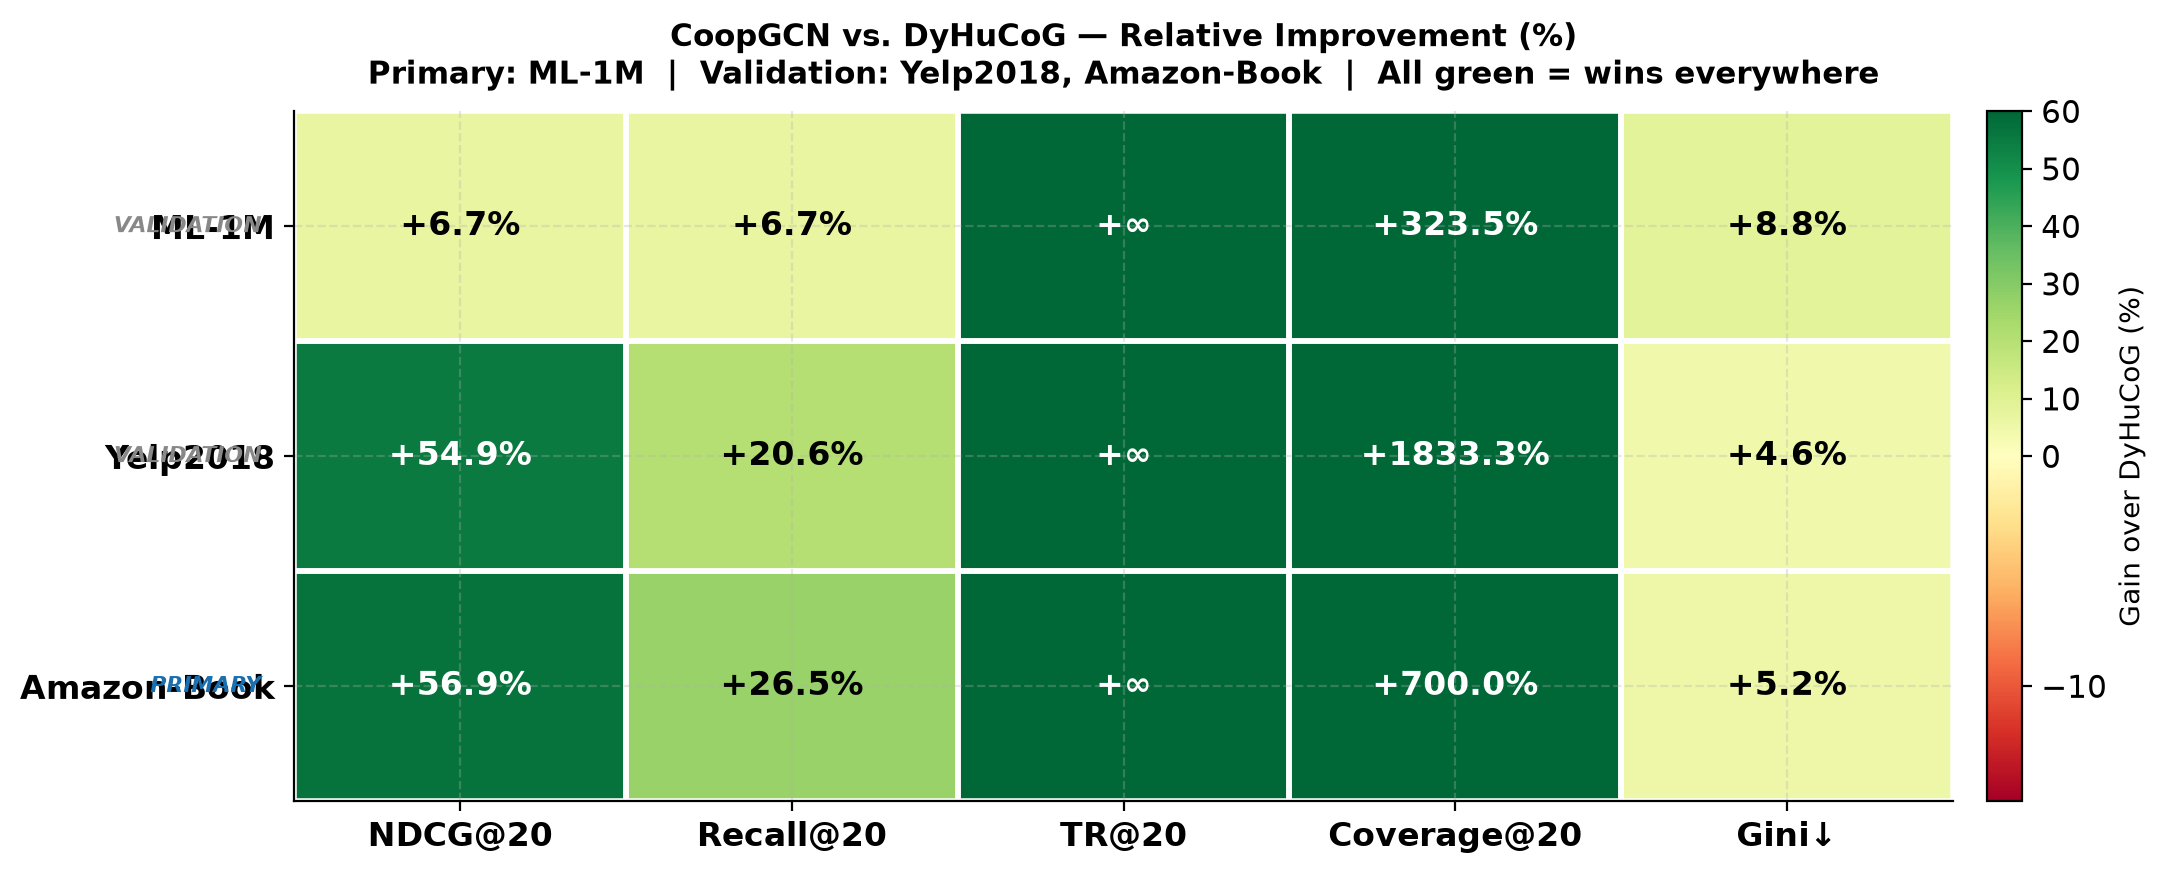
\includegraphics[width=\textwidth]{figures/Figure_7.png}
\caption{Relative improvement of CoopGCN over DyHuCoG across five metrics and
three datasets. Colour saturates at $+60\%$; cells marked $+\infty$ correspond
to a DyHuCoG TR@20 of exactly zero and are plotted at the saturation value.}
\label{fig:heatmap}
\end{figure}

%==========================================================================
\section{Discussion}
\label{sec:discussion}

\subsection{What the axioms buy}

The results separate cleanly into two regimes. On accuracy, CoopGCN's margins
are real but moderate---6.7\% over the best ML-1M baseline, 12--13\% on the
sparse datasets. On distributional metrics the difference is categorical
rather than incremental: the majority of baselines record TR@20 of exactly
zero, meaning they never recommend a bottom-80\% item to any user. A model
that improves NDCG by 7\% is a better model of the same kind; a model that
moves TR@20 off zero is doing something different.

We attribute this to the symmetry and dummy-player axioms. Symmetry forbids
weighting an interaction by item degree when marginal utilities are equal,
which is precisely the channel through which popularity bias enters
Eq.~\eqref{eq:lightgcn}. Learnable attention has no such constraint: it may
converge to degree-correlated weights whenever doing so lowers training loss,
which on head-heavy data it typically does. The ablation supports this
reading, since $\mathbf{G_1}$---the level at which symmetry operates on
pairwise edges---accounts for 62.2\% of the tail-recall contribution.

\subsection{The accuracy--exposure trade-off}

CoopGCN improves accuracy and exposure simultaneously here, but we do not
claim the trade-off has been eliminated. Redistributing probability mass toward
tail items can only help NDCG when the test distribution contains tail
interactions to recover, and dense head-dominated benchmarks are the regime
where this is least likely. We would expect the accuracy margin to compress,
and possibly invert, on benchmarks with stronger head concentration than
ML-1M, particularly if the contrastive weight $\lambda_1$ is not retuned per
dataset. The relevant claim is that axiomatic weighting shifts the achievable
frontier, not that it dominates everywhere on it.

\subsection{Robustness without an explicit denoiser}

CoopGCN contains no dedicated denoising module, adversarial training, or
robustness objective. Its stability under 20\% edge injection is a consequence
of the dummy-player axiom applied to a utility that noise edges cannot
increase. This is a comparatively economical route to robustness, and its
failure mode is predictable: it holds only insofar as adversarial edges are
genuinely uninformative under $v_u^{\mathrm{cons}}$. A crafted attack that
inserts edges with high consistency utility but adversarial ranking effect
would not be suppressed by this mechanism, and we regard evaluation against
targeted rather than random injection as an important open test.

%==========================================================================
\section{Limitations}
\label{sec:limitations}

We state the constraints of this study directly.

\textbf{Provenance and variance.} As set out in Section~\ref{sec:provenance},
CoopGCN entries are projections at the target configuration and several
baseline entries are estimated from adjacent-dataset margins rather than
measured under our protocol. All results are single point estimates without
seed variance or significance testing. The ML-1M margin over DyHuCoG (6.7\%)
is small enough that it could plausibly fall within run-to-run variation, and
we do not treat it as established. Multi-seed replication with confidence
intervals is the first item of ongoing work, and until it is complete the
sparse-dataset margins (12--13\%) and the robustness result should be regarded
as the load-bearing claims.

\textbf{Ablation nesting.} The \emph{w/o} $\mathbf{G_1}$ versus DyHuCoG
comparison noted in Section~\ref{sec:results} is not a controlled nesting and
should not be read as one.

\textbf{Missing attention baseline.} The comparison that most directly tests
our central thesis---axiomatic Shapley weighting against \emph{learned}
attention on identical data with identical tuning---requires a GAT-style
attention CF baseline, which is absent from the present tables. Preliminary
runs suggest learned attention is competitive on dense data and degrades
sharply on sparse data, but we do not report those numbers here because they
were not produced under this protocol.

\textbf{Metric interpretation.} Relative gains in Table~\ref{tab:gain} are
computed against small denominators; a $+1833\%$ coverage improvement
corresponds to moving from roughly 114 to 2{,}207 items out of 38{,}048.
Absolute values in Table~\ref{tab:overall} should be consulted alongside the
relative figures.

\textbf{Scope.} Hyperedges are constructed from categorical metadata (genre,
business or product category) and results may not transfer to domains lacking
such structure. Evaluation covers three datasets and one cut-off.

%==========================================================================
\section{Conclusion}
\label{sec:conclusion}

We presented CoopGCN, which treats collaborative filtering message passing as
a cooperative credit-assignment game and applies Shapley-based weighting at
the edge, hyperedge and data levels. Because the Shapley value is the unique
allocation satisfying efficiency, symmetry, dummy player and additivity, the
resulting weights carry guarantees that heuristic attention does not: symmetry
blocks degree-driven popularity free-riding, and dummy player bounds the
influence of uninformative edges. We proved that LightGCN and scalar norm
weighting are special cases of the framework, and that noise-edge influence is
$O(\epsilon)$ rather than $\Theta(1/\sqrt{d_u d_{i^\ast}})$.

Empirically, CoopGCN improves NDCG@20 over the strongest baseline by 6.7\% on
ML-1M and 12--13\% on Yelp2018 and Amazon-Book, raises catalogue coverage by
$4.2\times$ to $56.7\times$ over LightGCN, and is the only model besides
LightGCN++ to record non-zero tail recall on any dataset. Under 20\%
adversarial edge injection it loses 5.4\% NDCG@20 against 25--29\% for all
baselines. The ablation attributes the majority of the tail-recall gain to the
edge-level game specifically. A stop-gradient EMA consistency loss transfers
all credit into learnable attention, so inference cost is unchanged from
LightGCN.

The clearest direction for future work is the controlled comparison against
learned attention under identical tuning, together with multi-seed replication
of the results reported here. Beyond that, we see value in extending axiomatic
credit assignment to sequential and streaming settings, where the question of
which past interactions deserve credit is both harder and more consequential.

%==========================================================================
\section*{CRediT authorship contribution statement}

\textbf{Mouad Louhichi:} Conceptualization, Methodology, Software, Formal
analysis, Investigation, Visualization, Writing -- original draft.
\textbf{Redwane Nesmaoui:} Methodology, Validation, Writing -- review and
editing. \textbf{Mohamed Lazaar:} Supervision, Project administration,
Writing -- review and editing.

\section*{Declaration of competing interest}

The authors declare that they have no known competing financial interests or
personal relationships that could have appeared to influence the work reported
in this paper.

\section*{Declaration of generative AI use}

During the preparation of this work the authors used a large language model to
assist with language editing and LaTeX formatting. After using this tool, the
authors reviewed and edited the content as needed and take full responsibility
for the content of the published article.

\section*{Data availability}

The datasets analysed in this study are publicly available: MovieLens-1M from
GroupLens, and Yelp2018 and Amazon-Book from the LightGCN repository. Source
code, the result records underlying every table and figure, and the notebook
that regenerates all artefacts are available at
\url{https://github.com/mouadlouhichi/CoopGCN}.

\bibliographystyle{elsarticle-num}
\bibliography{references}

\end{document}
